\documentclass[conference]{IEEEtran}
\IEEEoverridecommandlockouts
\usepackage{cite}
\usepackage{amsmath,amssymb,amsfonts}
\usepackage{algorithmic}
\usepackage{graphicx}
\usepackage{textcomp}
\usepackage{xcolor}
\usepackage{tikz}
\usetikzlibrary{arrows.meta}
\usepackage{pgfplots}
\usepgfplotslibrary{groupplots}
\pgfplotsset{compat=1.18}
\usepackage{hyperref}
\hypersetup{colorlinks=true, linkcolor=black, citecolor=black, urlcolor=blue}
\usepackage{placeins}
\usepackage{multirow}
\usepackage{balance}
\def\BibTeX{{\rm B\kern-.05em{\sc i\kern-.025em b}\kern-.08em
    T\kern-.1667em\lower.7ex\hbox{E}\kern-.125emX}}
\begin{document}

\title{Mobility Diary: un sistema Context-Aware per il diario personale
di mobilità con Human Activity Recognition e privacy sulla posizione}

\author{\IEEEauthorblockN{Giacomo Bianco}
\IEEEauthorblockA{\textit{Dipartimento di Informatica} \\
\textit{Università di Bologna}\\
Bologna, Italia \\
\href{mailto:giacomo.bianco4@studio.unibo.it}{giacomo.bianco4@studio.unibo.it}}
}

\maketitle

\begin{abstract}
Questo lavoro presenta Mobility Diary, una piattaforma context-aware
che ricostruisce un diario personale di mobilità a partire da tracce
GPS e dati inerziali dello smartphone. Un modello di riconoscimento
delle attività individua la modalità di spostamento dell'utente,
mentre le posizioni ricorrenti vengono raggruppate automaticamente in
luoghi abituali con un'etichetta leggibile. La posizione dell'utente è
protetta da una tecnica di perturbazione spaziale, che genera una
vista privata dettagliata e una vista condivisibile meno precisa, con
un compromesso tra privacy e qualità del dato misurato
sperimentalmente. Il sistema include inoltre un assistente di percorso
sensibile al contesto, statistiche personali sulle abitudini di
mobilità e una dashboard web per il personale autorizzato. L'intera
piattaforma è containerizzata e avviabile con Docker Compose.
\end{abstract}

\begin{IEEEkeywords}
context-awareness, human activity recognition, location privacy, mobility diary
\end{IEEEkeywords}

\section{Introduzione}

Comprendere come le persone si muovono all'interno di un contesto urbano è
un problema di crescente interesse, con applicazioni che spaziano dalla
pianificazione dei trasporti alla progettazione di servizi personalizzati
per il singolo utente. Il semplice tracciamento della posizione, tuttavia,
non è sufficiente a cogliere il significato degli spostamenti: una
sequenza di coordinate GPS non distingue, ad esempio, tra un tragitto
percorso a piedi, in bicicletta o in automobile, né indica se un punto
visitato rappresenti un luogo rilevante per l'utente, come la propria
abitazione o il luogo di lavoro. Un sistema \emph{context-aware} per la
mobilità deve quindi andare oltre la semplice acquisizione di dati grezzi
di posizione, arricchendo la traccia con altre informazioni, 
quali l'attività di movimento riconosciuta e i luoghi significativi
frequentati, in modo da trasformare una sequenza di punti GPS in un
diario di mobilità realmente informativo.

In questo lavoro presento Mobility Diary, un sistema context-aware
composto da un'applicazione mobile per la raccolta dei dati di
mobilità, un back-end che ne gestisce l'elaborazione e la persistenza,
e una dashboard Web per la consultazione del diario. Il sistema integra
il riconoscimento dell'attività umana (Human Activity Recognition, HAR)
con meccanismi di protezione della privacy sui dati di posizione. Nello
specifico, il sistema realizza:
\begin{itemize}
    \item una pipeline di ingestione asincrona dei dati grezzi raccolti
    dal dispositivo mobile, basata su un pattern di caricamento diretto
    verso uno storage a oggetti (S3-compatible) seguito da una fase di
    conferma esplicita (\emph{direct-to-storage upload with confirm
    step}), che evita che i dati grezzi transitino dal server
    applicativo, seguito da un'elaborazione asincrona lato server che
    materializza la traccia di mobilità;
    \item la ricostruzione della mobilità dell'utente come sequenza di
    segmenti temporali, ciascuno associato a un luogo o a un'attività di
    movimento (cammino, bicicletta, automobile, sosta), a partire dalle
    tracce raccolte dal dispositivo;
    \item un modulo di Human Activity Recognition basato su una pipeline
    a due fasi CNN1D + GRU bidirezionale, addestrata sul dataset
    pubblico SHL (Sussex-Huawei Locomotion)~\cite{wang2018shl} per riconoscere cinque
    modalità di mobilità (\emph{idle}, \emph{walking}, \emph{running},
    \emph{biking}, \emph{moving vehicle}), con un'accuratezza dell'84,88\%
    sul validation set ufficiale dopo l'ottimizzazione del modello per
    l'inferenza in produzione;
    \item la generazione di viste privacy-aware del diario a tre livelli
    (\emph{precise}, \emph{approximate}, \emph{aggregated}), ottenute
    tramite una tecnica di generalizzazione spaziale a griglia (spatial
    cloaking) sulle tracce GPS, con valutazione quantitativa del
    compromesso tra perturbazione della posizione e qualità del servizio
    (Privacy Perturbation e Quality of Service).
\end{itemize}

Il resto dell'articolo è organizzato come segue: la Sezione~\ref{sec:architecture}
descrive l'architettura del sistema, la Sezione~\ref{sec:implementation}
ne dettaglia l'implementazione e la Sezione~\ref{sec:results} presenta i
risultati sperimentali ottenuti.

\section{Architettura del sistema}
\label{sec:architecture}

\subsection{Panoramica}

Il sistema è composto da due client -- l'applicazione mobile e la
dashboard Web -- e da un back-end raggiungibile attraverso un unico
gateway, come mostrato in Fig.~\ref{fig:architecture}. Il back-end
gestisce sia le operazioni sincrone del diario, sia l'elaborazione
asincrona dei dati grezzi caricati dal dispositivo, descritte nel
dettaglio nelle sottosezioni seguenti. Il dato nasce sul dispositivo
dell'utente, viene caricato verso il back-end e sottoposto a
un'elaborazione asincrona che ne estrae informazioni di contesto
(attività riconosciuta, luoghi significativi); viene infine
persistito e reso disponibile in lettura, con o senza protezione
della privacy, alla dashboard Web.

\begin{figure*}[t]
\centering
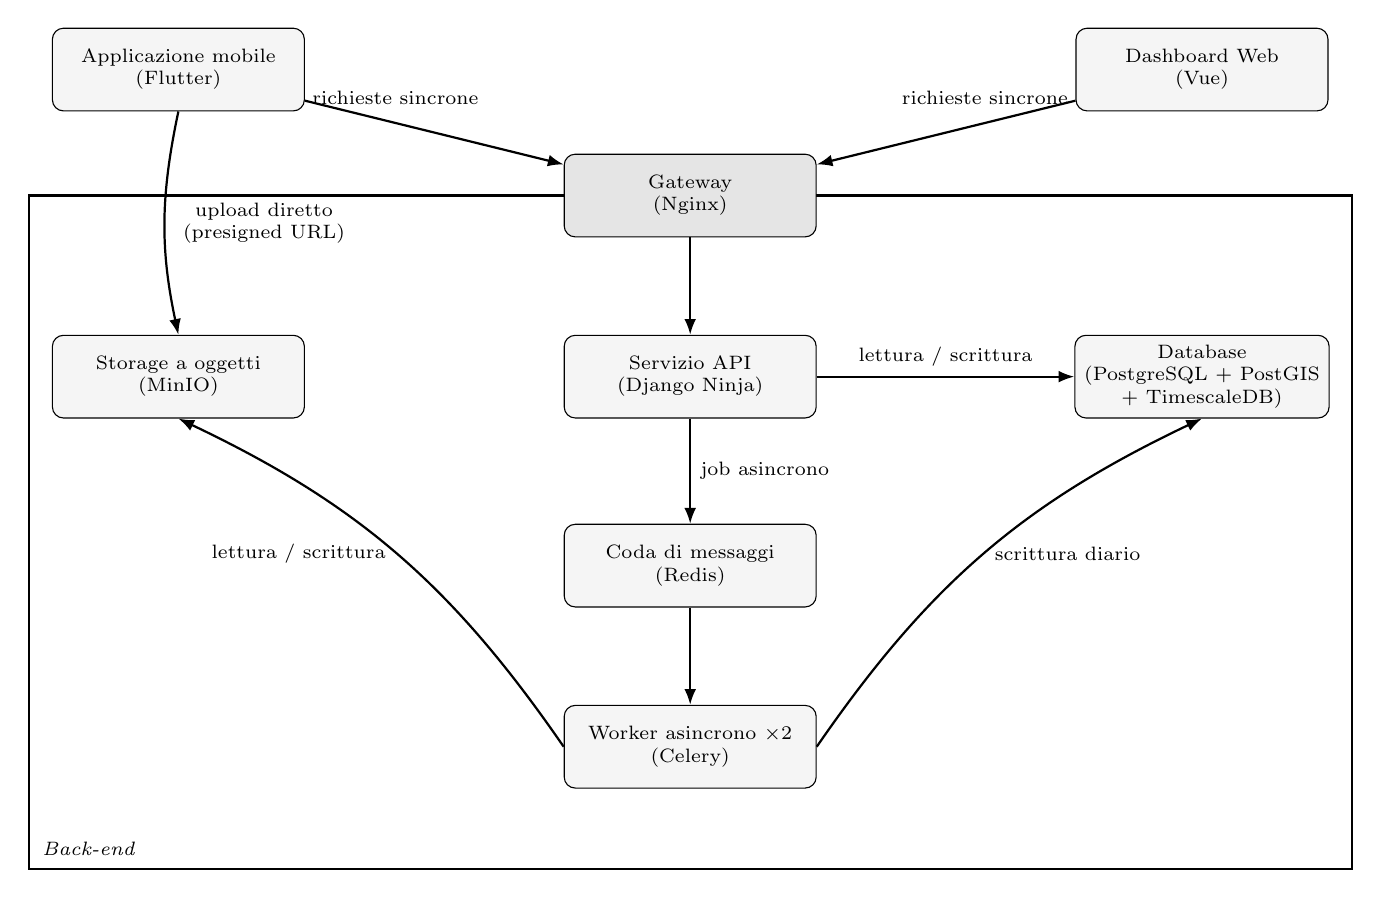
\begin{tikzpicture}[
  block/.style={draw, rounded corners, minimum width=3.2cm,
    minimum height=1.05cm, align=center, fill=gray!8},
  arrow/.style={-{Latex[length=2mm]}, thick},
  every node/.style={font=\scriptsize}
]

% Nodi esterni al back-end
\node[block] (mobile) at (0,9.6) {Applicazione mobile\\(Flutter)};
\node[block] (dashboard) at (13,9.6) {Dashboard Web\\(Vue)};

% Rettangolo di dominio: tutto il back-end, con il gateway sul bordo
\draw[thick] (-1.9,-0.55) rectangle (14.9,8);
\node[anchor=south west] at (-1.85,-0.5) {\scriptsize\textit{Back-end}};

\node[block, fill=gray!20] (gateway) at (6.5,8) {Gateway\\(Nginx)};

\node[block] (api) at (6.5,5.7) {Servizio API\\(Django Ninja)};
\node[block] (storage) at (0,5.7) {Storage a oggetti\\(MinIO)};
\node[block] (db) at (13,5.7) {Database\\(PostgreSQL + PostGIS\\+ TimescaleDB)};

\node[block] (redis) at (6.5,3.3) {Coda di messaggi\\(Redis)};

\node[block] (worker) at (6.5,1) {Worker asincrono $\times 2$\\(Celery)};

\draw[arrow] (mobile) -- (gateway) node[pos=0.35, above, yshift=1mm] {\scriptsize richieste sincrone};
\draw[arrow] (dashboard) -- (gateway) node[pos=0.35, above, yshift=1mm] {\scriptsize richieste sincrone};
\draw[arrow] (mobile.south) to[bend right=12] node[midway, right, align=center, xshift=1mm] {\scriptsize upload diretto\\(presigned URL)} (storage.north);
\draw[arrow] (gateway) -- (api);
\draw[arrow] (api) -- (db) node[midway, above] {\scriptsize lettura / scrittura};
\draw[arrow] (api) -- (redis) node[midway, right] {\scriptsize job asincrono};
\draw[arrow] (redis) -- (worker);
\draw[arrow] (worker.west) to[bend right=15] node[midway, left] {\scriptsize lettura / scrittura} (storage.south);
\draw[arrow] (worker.east) to[bend left=15] node[midway, right] {\scriptsize scrittura diario} (db.south);

\end{tikzpicture}
\caption{Architettura ad alto livello del sistema.}
\label{fig:architecture}
\end{figure*}

\subsection{Applicazione mobile}

L'applicazione mobile, sviluppata in Flutter, è responsabile della
raccolta dei dati sul dispositivo dell'utente. Localmente, l'applicazione
determina in autonomia se l'utente è in movimento o fermo, tramite una
macchina a stati finiti alimentata dai dati dei sensori, in modo da
adattare la frequenza di campionamento in base allo stato ed evitare un'acquisizione
continua e costante che porterebbe ad un consumo eccessivo della batteria. I dettagli di questa macchina a stati sono
discussi nella Sezione~\ref{sec:implementation}.

\subsection{Livello di ingresso e servizio applicativo}

Le richieste sincrone dell'applicazione mobile e della dashboard
attraversano un'unica istanza di gateway (Nginx), che instrada il
traffico verso il servizio applicativo, realizzato in Django con
Django Ninja e replicato su due istanze per poter servire richieste
concorrenti.
Questo livello espone le principali operazioni sincrone del sistema:
autenticazione dell'applicazione mobile e della dashboard, lettura del
diario giornaliero e delle tracce di mobilità, gestione dei luoghi
significativi (conferma, rifiuto, etichettatura), consultazione delle
statistiche personali, gestione delle preferenze di privacy ed
esportazione privacy-aware del diario, oltre alla gestione degli
utenti lato dashboard. È inoltre responsabile di schedulare nella coda
di messaggi i task relativi alle operazioni che richiedono
un'elaborazione asincrona.

\subsection{Pipeline di ingestione ed elaborazione}
\label{sec:architecture-pipeline}

Il caricamento dei dati grezzi raccolti dal dispositivo non avviene
attraverso il servizio applicativo, ma tramite un pattern di
caricamento diretto verso uno storage a oggetti, seguito da una fase di
conferma esplicita verso il back-end. Questa scelta evita che il
servizio applicativo non debba occuparsi del trasferimento di dati che potrebbero
occupare a lungo le sue connessioni, saturandone la capacità di
servire richieste concorrenti: il suo ruolo si limita ad autorizzare
il caricamento e a confermarne il completamento, mentre il
trasferimento dei dati avviene direttamente tra dispositivo e
storage.

Una volta confermato il caricamento, il dato viene preso in carico dal
livello di elaborazione asincrona (Celery), disaccoppiato dal servizio
applicativo tramite una coda di messaggi (Redis).
L'elaborazione avviene in quattro
fasi in sequenza, ciascuna dipendente
dall'output della precedente:
\subsubsection{Classificazione dell'attività}

Etichetta le
finestre di dati sensoriali presenti nello storage con la modalità di movimento
riconosciuta.

\subsubsection{Inserimento nel diario}

Materializza la traccia
di mobilità, i relativi segmenti e le etichette di movimento a
partire dai dati caricati e dalle etichette prodotte al passo
precedente.

\subsubsection{Inserimento batch dei dati sensoriali}

Persiste
le misure grezze nel database (TimescaleDB).

\subsubsection{Analisi dei luoghi abituali}

Individua i
luoghi significativi frequentati dall'utente a partire dai dati di
posizione inseriti nel diario.

La natura asincrona di queste quattro fasi permette di gestire
carichi di lavoro computazionalmente costosi (in particolare fase 1 e fase 3) senza impattare la latenza delle richieste
sincrone del servizio applicativo. I dettagli realizzativi di ciascuna
fase sono discussi nella Sezione~\ref{sec:implementation}.

\subsection{Persistenza}

Il sistema utilizza due meccanismi di persistenza distinti, scelti in
base alla natura del dato. I dati strutturati del diario, ovvero tracce,
segmenti, luoghi significativi ed etichette di attività, sono
memorizzati in un database relazionale esteso con PostGIS~\cite{postgis-manual}
e TimescaleDB~\cite{timescale-hypertables}, che permettono di eseguire query
geografiche e query di analisi pesanti basate su aggregazioni. 
I dati grezzi provenienti dai sensori, che non necessitano di essere
interrogati singolarmente ma solo recuperati per intero durante
l'elaborazione asincrona, sono invece mantenuti in uno storage a
oggetti separato dal database.

\subsection{Modello dei dati}

Le entità richieste dalla traccia sono rappresentate nel modello
persistente con i nomi riportati nella Tabella~\ref{tab:domain-model}.
La separazione tra traccia, segmenti e luoghi consente di conservare
l'evidenza grezza e di ricostruire una vista del diario aggiornata
quando cambiano le etichette dei luoghi.

\begin{table*}[htbp]
\caption{Corrispondenza tra le entità della traccia e il modello implementato}
\centering
\scriptsize
\begin{tabular}{|p{2.7cm}|p{3.7cm}|p{9.2cm}|}
\hline
\textbf{Entità concettuale} & \textbf{Modello implementato} & \textbf{Significato e attributi principali} \\
\hline
\texttt{MobilityTrace} & \texttt{Trip}, \texttt{GpsPoint} &
Un \texttt{Trip} delimita una sessione di mobilità e conserva stato,
intervallo temporale, distanza e percorso \texttt{LineString}. I
\texttt{GpsPoint} mantengono timestamp, coordinata PostGIS, velocità e
accuratezza della misura. \\
\hline
\texttt{MobilitySegment} & \texttt{MobilitySegment} &
Una riga persistente del diario, di tipo \texttt{MOVE} o \texttt{STOP},
con inizio, fine, attività riconosciuta, distanza e percorso opzionale. \\
\hline
\texttt{SignificantPlace} & \texttt{HabitualPlace} e \texttt{CandidateVisit} &
Una \texttt{CandidateVisit} rappresenta una singola permanenza; visite
spazialmente ricorrenti vengono aggregate in un \texttt{HabitualPlace},
con centro, raggio, conteggi, stato di revisione, categoria e nome scelto
dall'utente. \\
\hline
\texttt{ActivityLabel} & \texttt{ActivityLabel} &
Vocabolario controllato condiviso dai segmenti e dal classificatore:
\texttt{IDLE}, \texttt{WALKING}, \texttt{RUNNING}, \texttt{BIKING} e
\texttt{MOVING\_VEHICLE}. \\
\hline
\end{tabular}
\label{tab:domain-model}
\end{table*}

I campioni inerziali sono inoltre conservati in
\texttt{RawSensorReading}; le transizioni della macchina a stati in
\texttt{StateTransition}; lo stato della lavorazione asincrona in
\texttt{HarJob} e \texttt{TripUpload}. Queste entità sono operative e
non modificano il vocabolario di dominio richiesto dalla traccia.

\subsection{API REST}

L'app mobile usa token Bearer distinti dalle credenziali staff della
dashboard. Tutte le risposte applicative sono JSON; le geometrie sono
serializzate come GeoJSON in coordinate WGS84. La
Tabella~\ref{tab:rest-api} riassume gli endpoint principali; la specifica
OpenAPI completa e interattiva è pubblicata in \texttt{/api/docs}.

\begin{table*}[htbp]
\caption{Principali API REST usate dall'applicazione e dalla dashboard}
\centering
\scriptsize
\begin{tabular}{|p{3.8cm}|p{1.1cm}|p{4.7cm}|p{6cm}|}
\hline
\textbf{Endpoint} & \textbf{Metodo} & \textbf{Input principale} & \textbf{Output principale} \\
\hline
\texttt{/api/upload/trips/start} & POST &
Identificativo sessione client, dispositivo e timestamp iniziale &
Identificativo upload e stato della sessione idempotente \\
\hline
\texttt{/api/upload/trips/core} & POST &
Upload id, punti GPS e transizioni FSM &
Trip id, stato delle fasi core/raw e disponibilità della mappa \\
\hline
\texttt{/api/upload/trips/}\newline
\texttt{\{id\}/parts/*} & POST &
Numero parte, dimensione, checksum e conferma dell'upload &
URL firmata S3 oppure stato della parte; la chiusura accoda l'HAR \\
\hline
\texttt{/api/mobility/trips/}\newline
\texttt{\{id\}/track} & GET & Trip id &
Numero punti, distanza e traccia \texttt{LineString} GeoJSON \\
\hline
\texttt{/api/mobility/trips/}\newline
\texttt{\{id\}/diary} & GET & Trip id &
Stato di elaborazione e segmenti con intervallo, attività, distanza,
percorso e luogo associato \\
\hline
\texttt{/api/mobility/trips/}\newline
\texttt{\{id\}/privacy-export} & GET &
Trip id; il livello proviene dalle preferenze utente &
Diario condivisibile, coordinate pubblicate, dimensione cella e testo \\
\hline
\texttt{/api/mobility/places} & GET & Utente autenticato &
Luoghi candidati/confermati, categorie e visite di evidenza \\
\hline
\texttt{/api/mobility/analytics} & GET &
\texttt{granularity=day|week} & Bucket temporali, modalità prevalente,
rotte frequenti e, per la vista settimanale, heatmap \\
\hline
\texttt{/api/mobility/}\newline
\texttt{route-assistant/classify} & POST &
Matrice $500\times6$ di accelerometro e giroscopio &
Modalità di routing e confidenza della predizione \\
\hline
\texttt{/api/web/users/...} & GET &
Utente o trip id e filtri temporali/stato &
Proiezioni staff di utenti, viaggi, diario, privacy e statistiche sensore \\
\hline
\end{tabular}
\label{tab:rest-api}
\end{table*}

\subsection{Dashboard}

La dashboard Web, realizzata in Vue, non è pensata per l'utente
finale ma per un amministratore: consente di selezionare un utente da
un elenco e di ispezionarne il diario di mobilità a fini di supporto e
verifica. Consuma le API sincrone esposte dal servizio applicativo per
mostrare, per l'utente selezionato, le tracce di mobilità e i luoghi
significativi su mappa, il diario giornaliero in forma tabellare e
temporale, e le statistiche aggregate sulle attività riconosciute
prodotte dalla fase di data mining della pipeline. Permette inoltre
di confrontare la traccia reale con la corrispondente vista
privacy-aware, e di filtrare i dati mostrati per giorno, attività
riconosciuta, viaggio o intervallo temporale.

\subsection{Containerizzazione}

L'intera piattaforma server è avviabile con Docker Compose. Un gateway
Nginx costituisce l'unico ingresso HTTP e instrada \texttt{/api},
\texttt{/admin} e i file statici verso Django, gli oggetti caricati verso
MinIO e le restanti richieste verso la single-page application Vue,
compilata in uno stadio Node e servita da un container Nginx dedicato.
Completano lo stack PostgreSQL con PostGIS, Redis, i worker Celery, il
job di migrazione e il job di inizializzazione del bucket MinIO. Health
check e dipendenze di avvio impediscono al gateway di ricevere traffico
prima che dashboard, API, database e code siano disponibili. In ambiente
locale l'intera piattaforma viene costruita e avviata con
\texttt{docker compose -f back-end/infra/docker-compose.yml up --build}.

\section{Implementazione}
\label{sec:implementation}

\subsection{Applicazione mobile}

L'intero codice dell'applicazione mobile è organizzato seguendo Pine,
un'architettura leggera per progetti Flutter che separa in layer
distinti la UI, la logica di presentazione (Cubit/BLoC), i repository
e i servizi esterni, con dipendenze che attraversano i layer in una
sola direzione~\cite{pine-architecture}. Le sottosezioni seguenti
descrivono i moduli applicativi costruiti sopra questa struttura.

\subsubsection{Macchina a stati finiti di rilevamento del movimento}

L'applicazione è pensata per restare in esecuzione anche per diverse
ore nell'arco della giornata, il che rende il consumo energetico un
vincolo di progettazione non trascurabile. Durante l'intero utilizzo,
il sistema mantiene attivi tre stream di sensori: accelerometro,
giroscopio e GPS. Per contenere il consumo energetico senza rinunciare
alla qualità del dato, l'applicazione mantiene localmente una macchina
a stati finiti che determina se l'utente è in movimento
(\texttt{movement}) o fermo (\texttt{stationary})
(Sezione~\ref{sec:architecture}), e associa a ciascuno dei due stati
un profilo di campionamento diverso, riducendo la frequenza di
acquisizione quando l'utente è fermo.

\begin{figure*}[t]
\centering
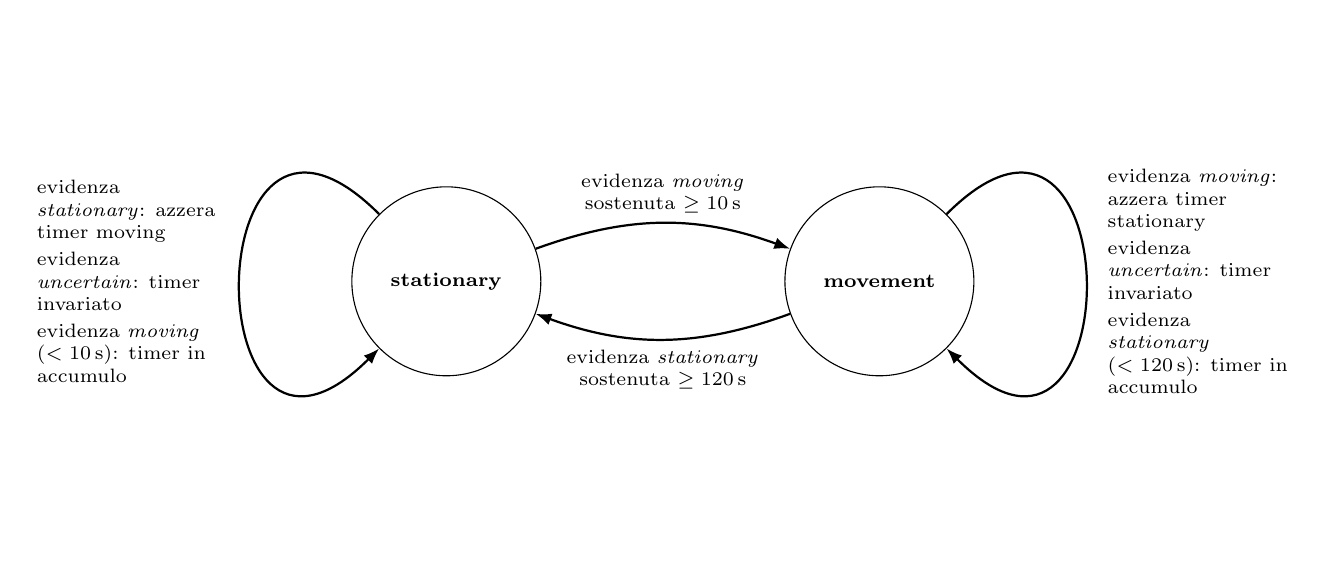
\begin{tikzpicture}[
  state/.style={draw, circle, minimum size=2.4cm, align=center},
  arrow/.style={-{Latex[length=2mm]}, thick},
  every node/.style={font=\scriptsize}
]

\node[state] (stationary) at (0,0) {\textbf{stationary}};
\node[state] (movement) at (5.5,0) {\textbf{movement}};

\draw[arrow] (stationary) to[out=135,in=225,looseness=5]
  node[left, xshift=-0.15cm]
  {\parbox{2.3cm}{\raggedright
   evidenza \emph{stationary}: azzera timer moving\\[2pt]
   evidenza \emph{uncertain}: timer invariato\\[2pt]
   evidenza \emph{moving} ($<10$\,s): timer in accumulo}}
  (stationary);

\draw[arrow] (movement) to[out=45,in=-45,looseness=5]
  node[right, xshift=0.15cm]
  {\parbox{2.3cm}{\raggedright
   evidenza \emph{moving}: azzera timer stationary\\[2pt]
   evidenza \emph{uncertain}: timer invariato\\[2pt]
   evidenza \emph{stationary} ($<120$\,s): timer in accumulo}}
  (movement);

\draw[arrow] (stationary) to[bend left=20] node[above, align=center]
  {evidenza \emph{moving}\\sostenuta $\geq 10$\,s} (movement);

\draw[arrow] (movement) to[bend left=20] node[below, align=center]
  {evidenza \emph{stationary}\\sostenuta $\geq 120$\,s} (stationary);

\end{tikzpicture}
\caption{Macchina a stati finiti di rilevamento del movimento: stati,
transizioni ed effetto di ciascun tipo di evidenza sui timer di
isteresi.}
\label{fig:fsm}
\end{figure*}

Per decidere se cambiare stato, la macchina osserva due valori: la
velocità istantanea fornita dal GPS e $\sigma$, la deviazione
standard della Signal Vector Magnitude (SVM) dell'accelerometro --
la SVM di un campione è $\sqrt{x^2+y^2+z^2}$ sulle tre componenti
dell'accelerazione. $\sigma$ non viene ricalcolato a ogni singolo
campione dell'accelerometro, ma accumulando i campioni in una
finestra e calcolandolo una sola volta al suo completamento: 20
campioni (2\,s a 10\,Hz) nello stato \texttt{stationary}, 500
campioni (5\,s a 100\,Hz, la stessa finestra usata per la
classificazione HAR) nello stato \texttt{movement}.

All'avvio di un viaggio la macchina viene inizializzata nello stato
\texttt{stationary}. In questo stato il profilo di campionamento
imposta l'accelerometro a 10\,Hz e disattiva il giroscopio (attivo
invece a 100\,Hz in \texttt{movement}, dove alimenta le finestre
sensoriali per la classificazione HAR); il GPS, in entrambi gli stati,
non campiona a una frequenza fissa ma emette un nuovo fix quando
l'utente si sposta di almeno 3\,m dall'ultima posizione nota. Una
soglia di spostamento più piccola produrrebbe un numero di fix
eccessivo rispetto alla precisione del GPS, che finirebbero comunque
tutti persistiti nel database, aumentando il volume di dati archiviati
senza un beneficio proporzionale sulla qualità della traccia. La
Tabella~\ref{tab:sensor-events} riassume la frequenza dei tre sensori
nei due stati, e dopo quanti dati ciascuno produce l'evento che fa
scattare una nuova valutazione della macchina a stati, cioè un nuovo
calcolo dell'evidenza (movimento, sosta o incerta) a partire dal dato
appena arrivato.

\begin{table}[htbp]
\caption{Frequenza dei sensori e generazione degli eventi per la
macchina a stati}
\centering
\scriptsize
\begin{tabular}{|l|p{1.1cm}|p{1.1cm}|p{2.6cm}|}
\hline
\textbf{Sensore} & \textbf{station.} & \textbf{movem.} & \textbf{Innesca una valutazione dopo} \\
\hline
Accelerometro & 10\,Hz & 100\,Hz & 20 campioni (2\,s) in \texttt{stationary}; 500 in \texttt{movement} (5\,s) \\
\hline
Giroscopio & spento & 100\,Hz & non alimenta la FSM: solo finestre HAR \\
\hline
GPS & a evento (3\,m) & a evento (3\,m) & immediato, a ogni fix \\
\hline
\end{tabular}
\label{tab:sensor-events}
\end{table}

Accelerometro e GPS sono quindi due processi indipendenti e asincroni:
ogni volta che uno dei due produce un nuovo dato, la macchina rivaluta
lo stato corrente combinando quel dato con l'ultimo valore noto
dell'altro segnale, entrambi soggetti a un controllo di freschezza
(rispettivamente 10\,s e 20\,s) che considera assente un dato più
vecchio della soglia. Il risultato di questa valutazione è
un'evidenza, movimento, sosta o incerta, ottenuta confrontando
$\sigma$ e la velocità GPS con soglie fisse.

Le soglie non sono le stesse in ogni situazione. Una velocità GPS pari
o superiore a 2.5\,m/s è considerata da sola sufficiente a dichiarare
evidenza di movimento, indipendentemente da $\sigma$, poiché
compatibile solo con un veicolo. Al di sotto di questa soglia, se lo
stato corrente è \texttt{movement} la decisione si basa solo su
$\sigma$: valori pari o superiori a 1.2 indicano movimento, valori
inferiori a 0.8 indicano sosta, i valori intermedi restano incerti.
Viene data priorità a $\sigma$ per due motivi legati fra loro: quando
la macchina a stati si trova in \texttt{movement} e deve stabilire se l'utente
si è davvero fermato, la sosta avviene tipicamente in un luogo chiuso,
dove il GPS diventa meno preciso; inoltre, se l'utente è realmente
fermo, il filtro di distanza di 3\,m descritto sopra fa sì che il GPS
smetta proprio di inviare nuovi dati.
Il segnale GPS quindi non solo perde precisione ma smette di
fornire nuova informazione proprio nel momento in cui servirebbe per
confermare la sosta, mentre l'accelerometro resta affidabile. Se
invece lo stato corrente è \texttt{stationary}, la
macchina a stati richiede che $\sigma$ e la velocità GPS concordino: evidenza
di movimento solo se $\sigma \geq 1.2$ e velocità $\geq 0.8$\,m/s,
evidenza di sosta solo se $\sigma < 0.8$ e velocità $< 0.5$\,m/s; in
tutti gli altri casi l'evidenza resta incerta. Questo requisito più
stringente nello stato \texttt{stationary} riduce i falsi positivi che
un singolo segnale rumoroso potrebbe generare quando l'utente è
effettivamente fermo: il sistema è pensato proprio per non segnalare
come movimento i piccoli spostamenti tipici di un ambiente chiuso,
come pochi passi in casa o in palestra.
A questo si aggiunge un vincolo temporale: le transizioni di stato
sono soggette a un tempo di conferma minimo asimmetrico, che richiede
un'evidenza sostenuta per un tempo minimo prima di confermare il
cambio di stato.
Questo è un ulteriore filtro contro i micro-spostamenti, che
raramente durano abbastanza a lungo da superarla. Da
\texttt{stationary} a \texttt{movement} sono richiesti 10\,s di
evidenza di movimento sostenuta, mentre da \texttt{movement} a
\texttt{stationary} ne sono richiesti 120\,s. Questa asimmetria evita
che una breve sosta durante uno spostamento (ad esempio a un semaforo)
chiuda prematuramente un
segmento di movimento. Ad ogni transizione, la macchina aggiorna il
profilo di campionamento dei sensori. Quando lo stato diventa
\texttt{movement}, il cambiamento è drastico: il filtro del GPS resta
invariato, ma il giroscopio si accende e accelerometro e giroscopio
passano entrambi a 100\,Hz. Questa frequenza non è arbitraria, ma
coincide con quella dei dati del dataset SHL usato per addestrare il
modello di Human Activity Recognition (Sezione~\ref{sec:implementation}),
poiché le finestre sensoriali raccolte in questo stato sono quelle
poi effettivamente classificate dal modello. La Fig.~\ref{fig:fsm}
riassume gli stati, le transizioni e tutti i casi di evidenza gestiti
dalla macchina.

\subsubsection{Rapporto tra macchina a stati e sistema HAR}

La macchina a stati e il sistema di Human Activity Recognition non
hanno lo stesso peso nella costruzione del diario: la macchina a stati
è la prima fonte di verità. Un segmento temporale che la macchina ha
classificato come \texttt{stationary} viene considerato sosta ed è
preso per buono come tale nel diario finale; il sistema HAR non
interviene su questi segmenti. Il suo ruolo si limita a classificare
la modalità di movimento all'interno dei soli intervalli di tempo che
la macchina a stati ha già decretato come \texttt{movement}.

Questa gerarchia si riflette direttamente su cosa viene persistito
localmente sul dispositivo. Le finestre di dati di accelerometro e
giroscopio, destinate alla classificazione HAR, vengono scritte nel
database locale (SQLite) solo durante le fasi in cui la macchina a
stati ha dichiarato \texttt{movement}: quando lo stato è
\texttt{stationary} i dati dei sensori (solo l'accelerometro, poiché
il giroscopio è spento) vengono usati esclusivamente per la decisione
della macchina stessa e non generano alcuna finestra da salvare. Questo non esclude che, all'interno di una finestra
classificata come \texttt{movement}, il sistema HAR possa poi
riconoscere sotto-intervalli in cui l'utente è di fatto fermo (ad
esempio una breve sosta a un semaforo); questo caso è discusso più
avanti (Sezione~\ref{sec:implementation}).

I dati del GPS seguono invece una logica diversa: vengono registrati
per tutta la durata del viaggio, incluse le fasi di sosta.
Vengono comunque sempre persistiti perché sono
necessari a ricostruire il viaggio nella sua interezza, anche dal
punto di vista grafico sulla mappa. La Fig.~\ref{fig:sensor-timeline}
riassume, lungo un viaggio composto da tre segmenti consecutivi, quali
dati vengono effettivamente persistiti localmente in SQLite in
ciascuna fase, prima di essere caricati e incorporati dal back-end
secondo la pipeline di ingestione descritta in
Sezione~\ref{sec:architecture-pipeline}.

\begin{figure}[htbp]
\centering
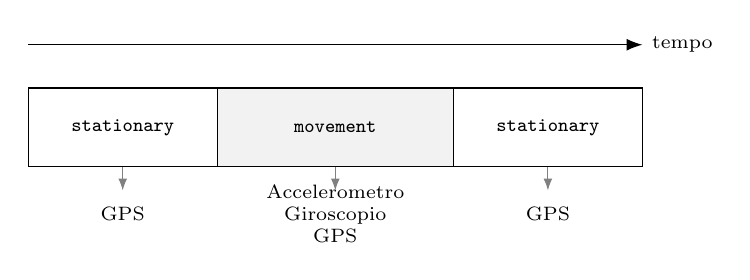
\begin{tikzpicture}[font=\scriptsize]

\draw[-{Latex[length=2mm]}] (0,1.55) -- (7.8,1.55) node[right] {tempo};

\draw (0,0) rectangle (2.4,1) node[midway] {\texttt{stationary}};
\draw[fill=gray!10] (2.4,0) rectangle (5.4,1) node[midway] {\texttt{movement}};
\draw (5.4,0) rectangle (7.8,1) node[midway] {\texttt{stationary}};

\node[align=center] at (1.2,-0.6) {GPS};
\node[align=center] at (3.9,-0.6) {Accelerometro\\Giroscopio\\GPS};
\node[align=center] at (6.6,-0.6) {GPS};

\draw[-{Latex[length=1.5mm]}, gray] (1.2,0) -- (1.2,-0.3);
\draw[-{Latex[length=1.5mm]}, gray] (3.9,0) -- (3.9,-0.3);
\draw[-{Latex[length=1.5mm]}, gray] (6.6,0) -- (6.6,-0.3);

\end{tikzpicture}
\caption{Dati persistiti localmente in SQLite lungo un viaggio
composto da tre segmenti: nelle fasi \texttt{stationary} viene
salvato solo il GPS, mentre nella fase \texttt{movement} vengono
salvati anche accelerometro e giroscopio, usati per la
classificazione HAR.}
\label{fig:sensor-timeline}
\end{figure}
\FloatBarrier

\subsubsection{Struttura e impacchettamento dei dati sensoriali per l'HAR}

Come descritto in Sezione~\ref{sec:architecture}, nello stato
\texttt{movement} accelerometro e giroscopio campionano entrambi a
100\,Hz. Ogni 5\,s di campioni viene raggruppato in una finestra,
ovvero una matrice $500 \times 6$: 500 campioni temporali per le sei
componenti Acc\_x, Acc\_y, Acc\_z, Gyr\_x, Gyr\_y, Gyr\_z. Localmente,
ogni finestra è persistita come una singola riga della tabella
\texttt{SensorWindows} del database SQLite: la matrice è serializzata
in formato JSON nella colonna \texttt{matrixJson}, accompagnata da
metadati (timestamp di inizio e fine, numero di campioni, frequenza).

Al momento della sincronizzazione, le finestre non vengono caricate
una alla volta né tutte insieme, ma raggruppate in più file. Le righe
della tabella vengono lette dal database a pagine di 128 finestre e
accumulate in un buffer finché la loro dimensione, misurata sul JSON
non compresso, non supera un budget di 12\,MB; a quel punto il buffer
viene scritto su un file e se ne apre uno nuovo. Ogni finestra pesa
circa 29\,KB da non compressa: il JSON è testo, e ogni valore viene
prima arrotondato a sei decimali, ad esempio per una singola riga a
sei canali:
\begin{quote}
\texttt{[-0.023457,-9.806649,0.112346,\allowbreak
0.001235,-0.004321,0.000765]}
\end{quote}
Con valori di questa forma, una
riga pesa circa 58 caratteri (51 per i sei numeri più 7 tra virgole e
parentesi), pari a circa 58 byte in UTF-8, dove ogni cifra o simbolo
occupa esattamente un byte; su 500 righe per finestra si ottengono
circa 29\,000 byte, coerenti con il valore osservato. Un file da
12\,MB contiene quindi approssimativamente 430 finestre (circa 36
minuti di registrazione).
Questo budget è tenuto volutamente basso per limitare il picco di
memoria della serializzazione sul telefono, indipendentemente dalla
durata complessiva del viaggio.

Ogni file viene poi compresso con GZIP, un formato di compressione
senza perdita basato sull'algoritmo DEFLATE: riduce la dimensione del
file individuando e codificando in modo più compatto le ripetizioni
nei dati, il che si adatta bene a un JSON con una struttura molto
regolare come questo, dimezzandone circa la dimensione (i 12\,MB non
compressi diventano circa 5\,MB). L'intera operazione, ovvero compressione
e calcolo del checksum SHA-256, viene eseguita in un isolate
separato dall'interfaccia utente, il meccanismo di Flutter per
eseguire codice su un thread indipendente, questo evita che un calcolo pesante come questo
possa bloccare il rendering dell'interfaccia.
Il checksum calcolato serve alla successiva fase di
conferma dell'upload (Sezione~\ref{sec:implementation}): la stringa
SHA-256 calcolata localmente viene inviata al back-end insieme al
file, che la confronta con il checksum calcolato sul file
effettivamente ricevuto sullo storage, per verificare che
corrispondano.

\subsubsection{Coda di sincronizzazione offline}

I dati raccolti localmente vengono sincronizzati verso il back-end
attraverso la tabella \texttt{SyncJobs} del database SQLite locale,
un record della quale gestisce di fatto una coda di sincronizzazione:
ogni sessione di raccolta genera un job, elaborato in ordine
cronologico -- i più vecchi per primi -- uno alla volta, per evitare
di saturare la connessione con più sessioni in parallelo.

Il caricamento di ogni job avviene in due fasi. Nella fase
\emph{core}, i punti GPS raccolti e i cambiamenti di stato tra
\texttt{movement} e \texttt{stationary} vengono inviati con una
richiesta diretta al servizio API, senza passare per lo storage a
oggetti. Nella fase \emph{raw}, vengono invece caricati i file
prodotti come descritto nella sottosezione precedente, secondo il
pattern di caricamento diretto con conferma descritto in
Sezione~\ref{sec:architecture-pipeline}: ciascuna parte viene prima
autorizzata dal back-end, poi caricata e infine confermata con il
relativo checksum. Ogni job traccia separatamente lo stato delle due
fasi, che possono essere confermate e ritentate in modo indipendente;
le parti raw vengono caricate a gruppi di tre in parallelo, anziché
una alla volta, per ridurre il tempo complessivo di sincronizzazione.

La coda gestisce esplicitamente i casi in cui il back-end sta ancora
elaborando in modo asincrono i dati ricevuti, mettendo il job in attesa
e ripetendo il controllo dello stato a intervalli regolari. In caso di
errore, il job viene ritentato con un ritardo crescente (10\,s, 30\,s,
2\,min, 10\,min) fino a un massimo di cinque tentativi, oltre i quali
viene scartato; un job scartato per cui il back-end ha già creato una
traccia viene inoltre annullato lato server, per non lasciare dati
parziali orfani. Al completamento con successo, i file temporanei
locali vengono eliminati e la sessione viene rimossa dal database
locale, mantenendo limitato lo spazio occupato sul dispositivo.

\subsubsection{Vincolo di un viaggio attivo alla volta}

Il sistema è pensato attorno a un'unica linea temporale per utente: il
diario è una sequenza di viaggi consecutivi, e non ha senso, in questo
modello, che due viaggi risultino in corso nello stesso momento. Questo
vincolo è realizzato facendo sì che, nel momento in cui l'utente preme
Start, venga già creato lato back-end un record del viaggio -- con
data di inizio e dispositivo associato -- anche se in quel momento i
dati non vengono ancora inviati: l'invio effettivo di tracce GPS e
dati sensoriali non è progressivo durante la registrazione, ma avviene
tutto in blocco solo alla pressione di Stop, secondo la coda di
sincronizzazione descritta in precedenza.

L'esistenza di questo record fin dall'avvio è ciò che permette di far
rispettare il vincolo: se l'utente prova ad avviare un nuovo viaggio da
un dispositivo diverso mentre, sullo stesso account, un viaggio
risulta già avviato e non ancora concluso, il back-end rifiuta la
richiesta con un conflitto, impedendo che due registrazioni si
sovrappongano sulla stessa linea temporale.

Durante il viaggio, l'applicazione invia inoltre al back-end un
segnale di \emph{heartbeat} ogni 5 minuti, che aggiorna un dato di
freschezza associato al viaggio in corso. Questo meccanismo protegge
da un caso limite: un viaggio che risulti ancora attivo ma che in
realtà non riceva aggiornamenti da troppo tempo.
Se un viaggio attivo resta senza heartbeat per più di 24 ore, viene chiuso
automaticamente non appena l'utente prova ad avviarne uno nuovo -- da
un altro dispositivo o dallo stesso -- permettendo alla registrazione
di ripartire anziché restare bloccata indefinitamente da un viaggio
ormai inattivo.

\subsubsection{Visualizzazione progressiva dei risultati}

Riprendendo le due fasi di caricamento (\emph{core} e \emph{raw}) e le
quattro fasi asincrone di elaborazione descritte in
Sezione~\ref{sec:architecture-pipeline}, l'applicazione mobile non
attende il completamento dell'intera pipeline per mostrare all'utente
il viaggio appena registrato. Non appena la fase \emph{core} è
confermata, l'applicazione mostra subito la mappa del viaggio nella
sua interezza, costruita a partire dai punti GPS caricati in quella
fase: è l'informazione più immediata da mostrare, ed è già disponibile
lato back-end a quel punto.

Per ottenere il diario con i segmenti colorati in base alla modalità
di movimento, l'applicazione effettua invece un polling verso il
back-end con cadenza di un secondo, richiedendo a ogni chiamata lo
stato di elaborazione del viaggio. Il back-end restituisce il diario
come completo solo quando il viaggio risulta processato, condizione
che si verifica nel momento in cui le fasi 1 e 2 della pipeline
asincrona -- classificazione dell'attività e inserimento nel diario --
sono terminate; le fasi 3 e 4 -- inserimento batch dei dati
sensoriali e data mining dei luoghi abituali -- non sono invece
necessarie per mostrare il diario e proseguono indipendentemente. Il
punto rilevante è quindi che l'utente non deve attendere il
completamento dell'intera elaborazione asincrona per vedere,
graficamente, l'esito del proprio viaggio, ma solo il termine delle
prime due fasi: questo riduce sensibilmente il tempo di caricamento
percepito rispetto all'attesa dell'intera pipeline. La
Fig.~\ref{fig:pipeline-timeline} riassume l'intera pipeline, dalla
pressione di Stop fino al completamento del data mining, insieme ai
due momenti in cui l'utente vede effettivamente qualcosa cambiare
nell'interfaccia.

\begin{figure*}[t]
\centering
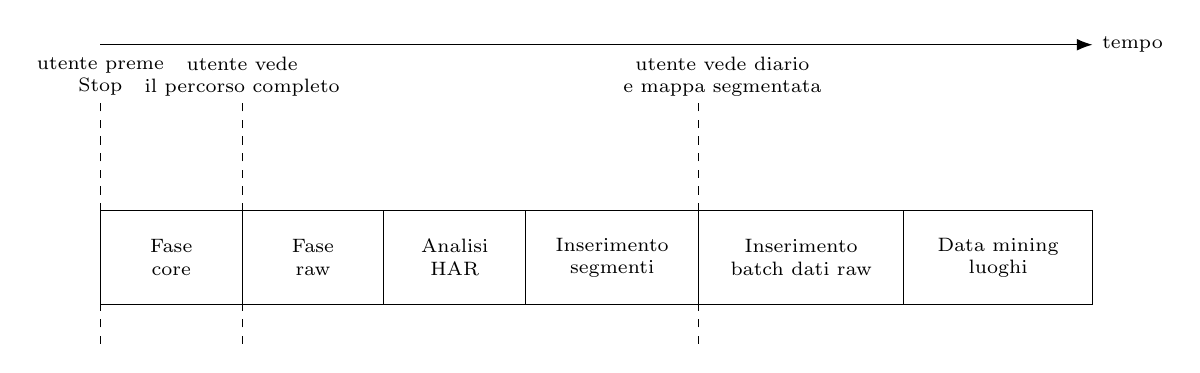
\begin{tikzpicture}[font=\scriptsize]

\draw[-{Latex[length=2mm]}] (0,3.3) -- (12.6,3.3) node[right] {tempo};

\draw (0,0) rectangle (1.8,1.2) node[midway, align=center] {Fase\\core};
\draw (1.8,0) rectangle (3.6,1.2) node[midway, align=center] {Fase\\raw};
\draw (3.6,0) rectangle (5.4,1.2) node[midway, align=center] {Analisi\\HAR};
\draw (5.4,0) rectangle (7.6,1.2) node[midway, align=center] {Inserimento\\segmenti};
\draw (7.6,0) rectangle (10.2,1.2) node[midway, align=center] {Inserimento\\batch dati raw};
\draw (10.2,0) rectangle (12.6,1.2) node[midway, align=center] {Data mining\\luoghi};

\draw[dashed] (0,-0.5) -- (0,2.6);
\node[align=center] at (0,2.9) {\scriptsize utente preme\\\scriptsize Stop};

\draw[dashed] (1.8,-0.5) -- (1.8,2.6);
\node[align=center] at (1.8,2.9) {\scriptsize utente vede\\\scriptsize il percorso completo};

\draw[dashed] (7.6,-0.5) -- (7.6,2.6);
\node[align=center] at (7.9,2.9) {\scriptsize utente vede diario\\\scriptsize e mappa segmentata};

\end{tikzpicture}
\caption{Pipeline completa di caricamento ed elaborazione.}
\label{fig:pipeline-timeline}
\end{figure*}

\subsubsection{Gestione dell'applicazione in background}

L'applicazione è pensata per un utilizzo prolungato nell'arco della
giornata: l'utente preme Start e lascia l'app in esecuzione, spesso in
background, per diverse ore. In questa condizione l'applicazione deve
gestire con attenzione sia il caso in cui il sistema operativo la
sospenda, sia più semplicemente il caso in cui l'utente non vi torni
per diversi minuti. La continuità della raccolta dati in questi stati
non è garantita allo stesso modo per tutti i sensori: i permessi di
localizzazione in background permettono di continuare a ricevere fix
GPS, ma le librerie usate per accelerometro e giroscopio non possono
garantire che i campioni continuino ad arrivare in ogni condizione di
background del sistema operativo.

Per questo motivo, quando l'utente torna nell'applicazione dopo
un'assenza, il sistema confronta i timestamp dell'ultima transizione
di stato, dell'ultimo punto GPS e dell'ultima finestra sensoriale
registrati localmente, e prende il più recente dei tre come istante
dell'ultima attività nota. Se da quell'istante sono trascorsi almeno
30 minuti, la sessione viene considerata autoconclusa: viene chiusa
retroattivamente, con istante di fine impostato a quell'ultima
attività nota anziché al momento della riapertura, e inviata al
back-end come se il viaggio si fosse concluso in quel momento. Se
invece sono trascorsi meno di 30 minuti, la sessione viene ripresa
normalmente. In questo caso, tuttavia, il sistema effettua una
correzione: se l'ultimo stato noto della macchina era
\texttt{movement}, ma nel frattempo i dati dei sensori hanno smesso di
arrivare, quel \texttt{movement} non è più considerato affidabile --
non essendoci conferma recente che l'utente sia ancora in movimento --
e il sistema forza lo stato a \texttt{stationary} a partire da quando
i dati si sono interrotti; la macchina a stati riprende quindi da
questo stato corretto, anziché dall'ultimo realmente osservato.

Questo meccanismo lato mobile, però, non basta da solo: può comunque
capitare che un segmento venga classificato dalla macchina a stati
come \texttt{movement}, ma che i dati sensoriali corrispondenti a
quell'intervallo non siano di fatto disponibili.
Per questo esiste un'ulteriore rete di
sicurezza lato back-end: quando, durante la costruzione del diario, un
segmento di movimento non ha finestre HAR classificate al suo interno,
il sistema non lo lascia privo di etichetta, ma stima l'attività a
partire dalla velocità mediana registrata dai punti GPS in
quell'intervallo, classificandola secondo soglie fisse (a piedi sotto
gli 8\,km/h, di corsa fino a 13\,km/h, in bicicletta fino a 25\,km/h,
altrimenti in veicolo).

\subsection{Route assistant context-aware}

L'assistente di percorso usa come punto A la posizione GPS corrente e
consente all'utente di cercare e selezionare un punto B tramite il
geocoding Mapbox. La richiesta Directions~\cite{mapbox-directions} usa uno dei tre profili
\texttt{walking}, \texttt{cycling} e \texttt{driving}; la risposta
GeoJSON viene mostrata sulla mappa insieme a distanza e durata stimate.
Il profilo può essere scelto manualmente oppure derivato dal modulo HAR:
\texttt{WALKING} e \texttt{RUNNING} diventano \texttt{walking},
\texttt{BIKING} diventa \texttt{cycling}, mentre
\texttt{MOVING\_VEHICLE} diventa \texttt{driving}.

Quando è attiva la modalità live, ogni 15 secondi il client preleva
l'ultima finestra inerziale $500\times6$ e la invia all'endpoint di
classificazione. Se la modalità riconosciuta cambia, lo stato del
client viene aggiornato e la rotta viene nuovamente richiesta usando il
profilo coerente. Il ricalcolo usa anche la posizione corrente più
recente, perciò reagisce sia a un cambio del mezzo sia allo spostamento
dell'utente. Contatori di generazione associati alle richieste di
geocoding e routing impediscono a risposte asincrone obsolete di
sovrascrivere una scelta più recente. La modalità può essere simulata
durante un replay, rendendo il cambio di percorso riproducibile nella
dimostrazione senza richiedere tre spostamenti reali differenti.

\subsection{Classificazione dell'attività (HAR)}

\subsubsection{Dataset e preparazione}

Il modulo HAR è addestrato sul dataset pubblico SHL (Sussex-Huawei
Locomotion)~\cite{wang2018shl}, raccolto con smartphone Huawei
indossati simultaneamente in quattro posizioni del corpo (tasca,
borsa, petto, mano). Ogni posizione registra a 100\,Hz accelerometro,
giroscopio e magnetometro, già pre-segmentati in finestre da 500
campioni (5\,s). Mescolare le quattro posizioni nel training rende il
modello robusto al fatto che, in un uso reale, non si sa dove l'utente
tenga il telefono.

Le otto classi originali del dataset (\texttt{IDLE}, \texttt{WALKING},
\texttt{RUNNING}, \texttt{DRIVING}, \texttt{BIKING}, \texttt{BUS},
\texttt{TRAIN}, \texttt{SUBWAY}) sono state ridotte a cinque, fondendo
le quattro modalità di trasporto motorizzato in un'unica classe
\texttt{MOVING\_VEHICLE}: le confusioni tra queste modalità erano
numerose (le firme inerziali di un'auto e di un mezzo pubblico sono
molto simili) e la fusione le trasforma da errori in predizioni
corrette, senza eliminare informazione utile al sistema, che non deve
distinguere tra mezzi di trasporto motorizzati diversi.

Le finestre consecutive distano solo 5\,s, quindi uno split casuale
porterebbe campioni quasi uguali in training e test (leakage
temporale). Il protocollo adottato usa il training set ufficiale,
riserva la sua ultima porzione temporale (15\%) all'early stopping e
impiega il validation set ufficiale solo per la valutazione finale.

\subsubsection{Architettura del modello}

Il classificatore di base è una CNN1D che scorre lungo il tempo,
leggendo tutti i canali dei sensori a ogni passo: due blocchi
convoluzione+pooling (\texttt{Conv1D(64)}, \texttt{Conv1D(128)}, kernel
10, con \texttt{MaxPooling1D}) seguiti da un \texttt{Dense(128)} e da
uno strato di uscita softmax sulle cinque classi, per circa 2 milioni
di parametri complessivi. Le convoluzioni sulle serie inerziali
multicanale seguono l'approccio di feature learning per HAR
di~\cite{yang2015cnn}.

Non vengono calcolate feature statistiche manuali come media, varianza,
energia, minimo o massimo. L'ingresso è la finestra grezza
$500\times6$ di accelerometro e giroscopio.

I filtri convoluzionali apprendono pattern locali discriminanti e il
livello denso li comprime in un embedding di 128 valori. La
GRU~\cite{cho2014gru} apprende le dipendenze tra gli embedding di
finestre consecutive.

Una normalizzazione per-canale, calcolata solo sul training set e
riapplicata a validation e test, e una \emph{focal loss} contrastano
lo sbilanciamento delle classi (\texttt{MOVING\_VEHICLE} è circa il
51\% dei dati, pesando di più gli esempi rari e quelli difficili).

Il contesto temporale è appreso, non imposto con una regola fissa: una
GRU bidirezionale legge sequenze di \emph{embedding} prodotti dalla
CNN su finestre consecutive (rispettando i confini tra le quattro
posizioni del corpo) e produce una predizione per ciascuna finestra
della sequenza, informata dal contesto passato e futuro.

Il confronto tra le varianti e le metriche del modello distribuito
sono riportati nella Sezione~\ref{sec:har-results}.

\subsubsection{Ottimizzazione per l'inferenza in produzione}

Il modello distribuito in produzione usa 6 canali (solo accelerometro
e giroscopio, senza magnetometro): quello dei telefoni reali si è
rivelato meno affidabile di quello del dataset SHL, tanto da rendere
preferibile ometterlo. La configurazione iniziale usava sequenze da 32
finestre; la valutazione quantitativa è riportata nei Risultati.

Nella pipeline a due fasi originale (CNN e GRU come due modelli
separati), l'inferenza in produzione mostrava tempi incoerenti e non
proporzionali al numero di finestre elaborate. L'analisi ha
individuato più cause concorrenti: la ricompilazione del grafo di
calcolo (\emph{graph retracing}) ogni volta che \texttt{model.predict()}
riceveva una dimensione di batch mai vista dal processo, costosa circa
2,3\,s per la rete CNN+GRU; un ciclo Python che chiamava la GRU una
volta per ogni gruppo di 32 finestre invece che con un'unica chiamata
sull'intero batch, circa 4,4 volte più lento; e uno stato
dell'ottimizzatore Adam rimasto nei checkpoint, inutile in inferenza e
responsabile di gran parte della loro dimensione su disco.

La soluzione applicata combina due interventi indipendenti. Primo, la
CNN e la GRU sono state fuse in un unico modello end-to-end, con i
pesi copiati (non riaddestrati) dai due checkpoint esistenti e
l'equivalenza numerica verificata rispetto alla pipeline originale
(differenza massima sulle probabilità dell'ordine di $10^{-7}$,
rumore numerico). Secondo, il modello fuso è avvolto in una
\texttt{tf.function} con una \texttt{input\_signature} esplicita a
batch dinamico ma lunghezza di sequenza fissa, così da forzare
un'unica compilazione valida per qualunque numero di finestre per
richiesta, eseguita una volta sola al posto di ripetersi a ogni nuova
dimensione di batch; una chiamata di riscaldamento all'avvio del
processo worker sposta questo costo di compilazione dalla prima
richiesta reale al momento dell'inizializzazione.

La lunghezza di sequenza della GRU, fissata a 32 finestre nella pipeline
originale, non era stata ritarata dopo il passaggio a sei canali.
La configurazione distribuita usa 128 finestre, scelta mediante la
valutazione riportata nella Sezione~\ref{sec:har-results}.

Il confronto di accuratezza e latenza tra pipeline originale e
ottimizzata è presentato nella stessa sezione.

\subsection{Inserimento nel diario e persistenza dei dati sensoriali}

\subsubsection{Rappresentazione geospaziale e query di distanza}

Tutti i dati geospaziali del sistema -- i punti GPS, il percorso di
ogni segmento, i centroidi delle visite e dei luoghi abituali -- sono
salvati nel database non come geometria piana, ma con il tipo
\texttt{geography} di PostGIS (coordinate WGS84, SRID 4326). Questa
scelta permette a PostGIS di calcolare le operazioni geospaziali
tenendo conto della curvatura della Terra, invece di trattare
latitudine e longitudine come coordinate su un piano: in particolare,
la lunghezza di un percorso salvato come \texttt{LineString} può
essere ottenuta con una singola funzione (\texttt{ST\_Length} su
geografia), che restituisce direttamente una distanza geodetica in
metri, senza che l'applicazione debba implementare a mano formule di
distanza tra coordinate. Questa funzione viene usata ripetutamente nel
sistema: per calcolare la distanza di ogni segmento di movimento
appena costruito, per confrontare la lunghezza di un percorso con
quella della sua versione privacy-aware (Sezione~\ref{sec:implementation}),
e più in generale ogni volta che serve una misura di distanza reale a
partire da una geometria salvata.

\subsubsection{Segmentazione del diario}

Nella prima fase di segmentazione del diario, il sistema usa le
transizioni della macchina a stati (Sezione~\ref{sec:implementation})
per individuare macro-intervalli \texttt{STOP}/\texttt{MOVE}: gli
intervalli \texttt{STOP} diventano segmenti di sosta senza bisogno di
ulteriore elaborazione, poiché la macchina a stati è già la fonte di
verità per la sosta. Gli intervalli \texttt{MOVE}, al contrario,
vengono affinati in un secondo passo usando le etichette prodotte dal
modulo HAR sulle finestre sensoriali che ricadono in quell'intervallo.

Questo affinamento applica due correzioni, a due scale temporali
diverse, per distinguere il rumore del classificatore da vere pause
nel movimento. La prima corregge cambi di etichetta isolati e brevi:
se un gruppo di finestre con un'etichetta diversa è compreso tra due
gruppi con la stessa etichetta e dura meno di 60\,s, viene riassegnato
all'etichetta circostante, assumendo che sia un errore di
classificazione piuttosto che un cambio di attività reale. La seconda
distingue le soste vere da quelle spurie all'interno di un movimento,
ed è motivata da un limite intrinseco della macchina a stati stessa:
per dichiarare una sosta, la macchina richiede almeno 120\,s di
evidenza di quiete sostenuta (Sezione~\ref{sec:implementation}).
Durante quei 120\,s, però, il dispositivo continua comunque a
raccogliere e classificare finestre sensoriali, ed è molto probabile
che il modulo HAR le etichetti correttamente come \texttt{IDLE},
perché l'utente è di fatto già fermo -- anche se il macro-segmento
costruito dalla macchina a stati etichetta ancora quell'intervallo
come \texttt{movement}, non avendo essa stessa completato la propria
isteresi. Per questo, un gruppo di finestre classificate
\texttt{IDLE} che dura abbastanza viene riconosciuto
come sosta reale e
diventa una \emph{pausa virtuale}; un \texttt{IDLE} più breve viene
invece assorbito nell'etichetta di movimento circostante, trattato
come rumore del classificatore. I gruppi risultanti, se adiacenti nel
tempo e con la stessa etichetta, vengono infine uniti in un unico
segmento (Fig.~\ref{fig:isolated-label}).

\begin{figure}[htbp]
\centering
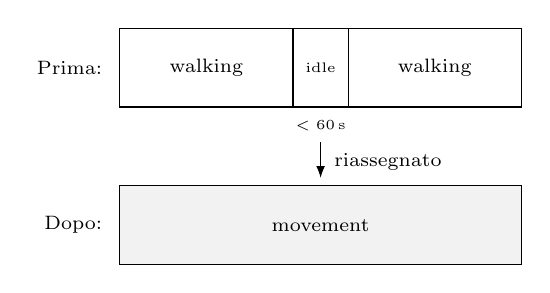
\begin{tikzpicture}[font=\scriptsize]

\node[anchor=east] at (-0.1,2.3) {Prima:};
\draw (0,1.8) rectangle (2.2,2.8) node[midway] {walking};
\draw (2.2,1.8) rectangle (2.9,2.8) node[midway] {\tiny idle};
\draw (2.9,1.8) rectangle (5.1,2.8) node[midway] {walking};
\node[below] at (2.55,1.75) {\tiny $<60$\,s};

\draw[-{Latex[length=1.5mm]}] (2.55,1.35) -- (2.55,0.9);
\node[right] at (2.6,1.1) {\scriptsize riassegnato};

\node[anchor=east] at (-0.1,0.3) {Dopo:};
\draw[fill=gray!10] (0,-0.2) rectangle (5.1,0.8) node[midway] {movement};

\end{tikzpicture}
\caption{Correzione di un cambio di etichetta isolato e breve (durata
$<60$\,s): il gruppo centrale viene riassegnato all'etichetta
circostante.}
\label{fig:isolated-label}
\end{figure}

La distinzione tra pausa virtuale e sosta vera resta interna alla
fase di segmentazione: nel diario finale mostrato all'utente le due
vengono trattate allo stesso modo, e unite in un'unica sosta
(Fig.~\ref{fig:virtual-stop-merge}).

\begin{figure}[htbp]
\centering
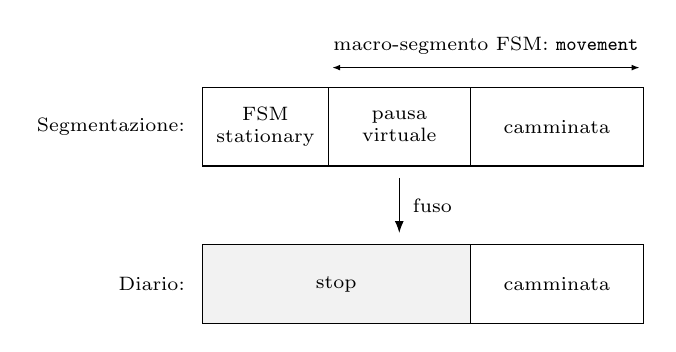
\begin{tikzpicture}[font=\scriptsize]

\node[anchor=east] at (-0.1,2.3) {Segmentazione:};
\draw (0,1.8) rectangle (1.6,2.8) node[midway, align=center] {FSM\\stationary};
\draw (1.6,1.8) rectangle (3.4,2.8) node[midway, align=center] {pausa\\virtuale};
\draw (3.4,1.8) rectangle (5.6,2.8) node[midway] {camminata};
\draw[{Latex[length=1mm]}-{Latex[length=1mm]}] (1.65,3.05) -- (5.55,3.05);
\node[above] at (3.6,3.1) {\scriptsize macro-segmento FSM: \texttt{movement}};

\draw[-{Latex[length=1.5mm]}] (2.5,1.65) -- (2.5,0.95);
\node[right] at (2.55,1.3) {\scriptsize fuso};

\node[anchor=east] at (-0.1,0.3) {Diario:};
\draw[fill=gray!10] (0,-0.2) rectangle (3.4,0.8) node[midway] {stop};
\draw (3.4,-0.2) rectangle (5.6,0.8) node[midway] {camminata};

\end{tikzpicture}
\caption{Una pausa virtuale rilevata dentro un macro-segmento
\texttt{movement} viene unita, nel diario finale, alla sosta
\texttt{stationary} adiacente decisa dalla FSM.}
\label{fig:virtual-stop-merge}
\end{figure}

\subsubsection{Persistenza dei dati sensoriali grezzi}

Una volta completata la costruzione del diario (fasi 1 e 2 della
pipeline, Sezione~\ref{sec:architecture-pipeline}), la terza fase
inserisce i dati sensoriali grezzi caricati dal dispositivo nel
database delle serie temporali. Qui ogni singolo campione di accelerometro e giroscopio diventa una riga a sé.

L'inserimento avviene tramite \texttt{bulk\_create} a blocchi di 5.000
righe. 
Il vantaggio di questa rappresentazione riga per campione si osserva nell'utilizzo
analitico che se ne fa.

\subsubsection{Utilizzo analitico dei dati sensoriali grezzi}

Inserire i dati grezzi riga per campione in un database rende possibile interrogarli
direttamente con query SQL.
Il sistema sfrutta questa possibilità per effettuare due analisi visibili dal pannello admin.

La prima query individua eventuali buchi anomali nella registrazione di un singolo viaggio:
va a confrontare ogni singolo campione di accelerometro e giroscopio con il precendete all'interno dello stesso segmento di movimento, 
segnalando intervalli temporali superiori a 10\,ms (considerando che i campioni sono acquisiti a una frequenza di 100 Hz). 

La seconda query calcola, per ciascuna modalità di attività riconosciuta, la media e la deviazione standard delle 
sei componenti di accelerometro e giroscopio, considerando tutti i viaggi dell’utente.

\subsection{Data mining dei luoghi abituali}

L'individuazione dei luoghi abituali avviene in due fasi successive:
prima un rilevamento delle soste (\emph{stay detection}) sui punti GPS
grezzi, poi un raggruppamento spaziale di queste soste in luoghi
ricorrenti tramite DBSCAN. La prima fase è necessaria perché DBSCAN,
di per sé, raggruppa i punti solo in base alla vicinanza spaziale e
non tiene conto della dimensione temporale: da solo non può distinguere
punti densi perché l'utente è rimasto fermo a lungo in un unico luogo
da punti densi perché l'utente vi è tornato più volte in giorni
diversi.

La prima fase scorre tutti i punti GPS di un utente in ordine temporale,
scartando quelli con precisione peggiore di 60\,m, e accumula un
cluster di punti consecutivi finché ciascun nuovo punto resta entro
75\,m dal centroide corrente del cluster e il tempo trascorso
dall'ultimo punto non supera i 90 minuti; al primo punto troppo
lontano o dopo un buco temporale troppo lungo, il cluster viene chiuso
e se ne inizia uno nuovo. Un cluster diventa una \emph{visita}
candidata solo se contiene almeno 3 punti e copre almeno 5 minuti,
condizioni che scartano soste troppo brevi.

Le visite individuate vengono poi raggruppate spazialmente con
DBSCAN~\cite{ester1996dbscan}.
Per ogni cluster risultante vengono calcolati il centroide, il raggio (la distanza massima tra il
centroide e una visita del cluster) e il numero di giorni distinti in
cui è stata osservata una visita. Un cluster di punti individuato dal DBSCAN viene 
promosso a possibile luogo abituale solo se le visite coprono almeno 2 giorni distinti,
ed è promosso automaticamente a confermato quando ne raggiunge almeno 4,
altrimenti resta in attesa di revisione manuale da parte dell'utente
tramite la dashboard. La Fig.~\ref{fig:place-mining} riassume l'intera
pipeline, dai punti GPS grezzi al ciclo di vita del luogo abituale.

\begin{figure}[htbp]
\centering
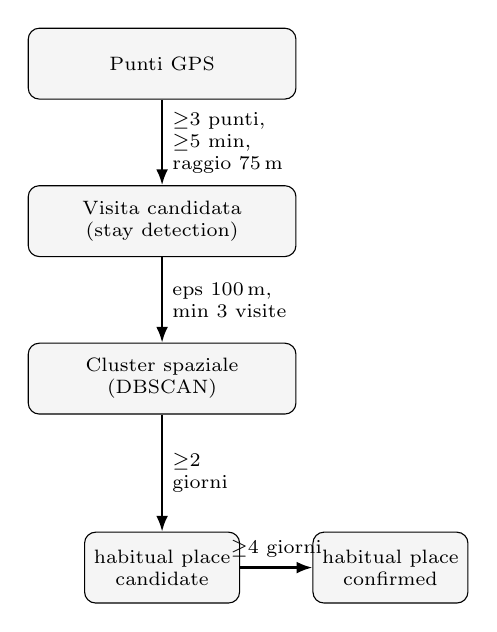
\begin{tikzpicture}[
  font=\scriptsize,
  block/.style={draw, rounded corners, minimum width=3.4cm,
    minimum height=0.9cm, align=center, fill=gray!8},
  arrow/.style={-{Latex[length=2mm]}, thick}
]

\node[block] (gps) at (0,8.0) {Punti GPS};
\node[block] (visit) at (0,6.0) {Visita candidata\\(stay detection)};
\node[block] (cluster) at (0,4.0) {Cluster spaziale\\(DBSCAN)};
\node[block, minimum width=1.8cm] (candidate) at (0,1.6) {habitual place\\candidate};
\node[block, minimum width= 1.9cm] (confirmed) at (2.9,1.6) {habitual place\\confirmed};

\draw[arrow] (gps) -- (visit) node[midway, right, align=left]
  {$\geq$3 punti,\\$\geq$5 min,\\raggio 75\,m};
\draw[arrow] (visit) -- (cluster) node[midway, right, align=left]
  {eps 100\,m,\\min 3 visite};
\draw[arrow] (cluster) -- (candidate) node[midway, right, align=left] {$\geq$2\\giorni};
\draw[arrow] (candidate) -- (confirmed) node[midway, above] {$\geq$4 giorni};

\end{tikzpicture}
\caption{Pipeline di individuazione dei luoghi abituali: dai punti GPS
grezzi alla stay detection, al raggruppamento DBSCAN, fino al ciclo di
vita candidate/confirmed del luogo.}
\label{fig:place-mining}
\end{figure}

I luoghi confermati vengono infine usati in lettura per arricchire il
diario: a ogni segmento di sosta (reale o pausa virtuale) viene
associato, se esiste, il luogo confermato più vicino al suo centroide
GPS.

Questa dipendenza in lettura ha una conseguenza diretta su come il
diario privato viene servito: non esiste, in senso stretto, una
versione definitiva e già pronta del diario da restituire, perché il
suo contenuto dipende anche dai luoghi abituali dell'utente, che
possono cambiare nel tempo indipendentemente dal viaggio stesso -- ad
esempio quando l'utente conferma, rifiuta o rietichetta un luogo dalla
dashboard. Per questo il diario privato è tenuto in una cache (Redis),
ma la chiave di cache include, oltre all'identificativo del viaggio,
un contatore di versione dei luoghi dell'utente: ogni revisione di un
luogo incrementa questo contatore, e la cache esistente diventa
automaticamente irraggiungibile con la nuova chiave, senza bisogno di
invalidarla esplicitamente. La richiesta successiva del diario trova
quindi la cache mancante e lo ricostruisce da zero, con le
associazioni ai luoghi aggiornate.

\subsection{Analitiche personali}

L'endpoint \texttt{/api/mobility/analytics} costruisce un'unica
risposta usata dalla pagina statistiche dell'app. Il parametro
\texttt{granularity} accetta \texttt{day} o \texttt{week}; il back-end
assegna timestamp e settimane nel fuso \texttt{Europe/Rome}, includendo
automaticamente il passaggio tra ora solare e legale. I bucket
giornalieri o settimanali sommano durata e distanza dei
\texttt{MobilitySegment} per ciascuna delle cinque etichette HAR. Il
client mostra al massimo sette bucket alla volta e consente di scorrere
l'intero storico con uno slider.

Le abitudini generali non dipendono dal bucket selezionato. La modalità
prevalente è l'attività non \texttt{IDLE} con durata storica totale
maggiore. Le rotte frequenti sono calcolate direttamente in PostGIS:
per ogni viaggio con una linea valida vengono estratti primo e ultimo
punto, associati al luogo confermato più vicino entro il massimo tra il
raggio del luogo e 150\,m, e infine raggruppati per coppia ordinata
origine--destinazione. Le coppie con stessa origine e destinazione sono
escluse e vengono restituite le cinque più frequenti.

Quando la granularità è settimanale, una seconda aggregazione PostGIS
restituisce tutte e sole le settimane storiche che contengono almeno un
viaggio, ordinate cronologicamente. Ogni settimana contiene gli id dei
viaggi e una heatmap dei luoghi confermati raggiunti alle estremità dei
percorsi; il peso di un luogo è il numero di viaggi distinti della
settimana che lo toccano. Un viaggio privo di path mantiene visibile la
settimana ma non contribuisce ai punti della heatmap. Con granularità
giornaliera questa query non viene eseguita. La pagina presenta inoltre
tempo totale in movimento, distanza, ripartizione per attività, modalità
prevalente e rotte frequenti.

\subsection{Modulo di privacy}

Delle tre viste del diario (\emph{precise}, \emph{approximate},
\emph{aggregated}, Sezione~\ref{sec:architecture}), solo le ultime due
applicano davvero una protezione: la vista \emph{precise} non è
sottoposta ad alcuna trasformazione ed espone le coordinate GPS
esattamente come raccolte, per cui non è un vero livello di privacy ma
la vista personale, non protetta, dell'utente sui propri dati. 
Le viste \emph{approximate} e
\emph{aggregated} sono ottenute con una generalizzazione spaziale
ispirata allo \emph{spatial cloaking}~\cite{gruteser2003cloaking}.
La variante usa una griglia deterministica e non dichiara le garanzie
di $k$-anonimato del metodo originale. Ogni coordinata
GPS viene proiettata in Web Mercator (EPSG:3857) e riposizionata al
centro della cella di una griglia di lato fisso a cui appartiene --
150\,m per la vista \emph{approximate}, 400\,m per
\emph{aggregated} -- prima di essere riproiettata in coordinate
geografiche, come mostrato in Fig.~\ref{fig:privacy-grid}.

\begin{figure}[htbp]
\centering
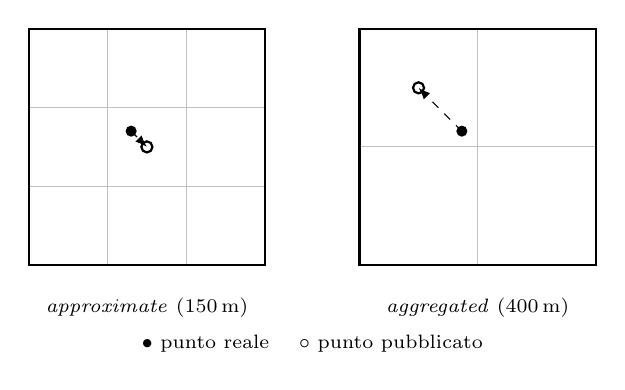
\begin{tikzpicture}[font=\scriptsize]

\draw[step=1cm, gray!50, thin] (0,0) grid (3,3);
\draw[thick] (0,0) rectangle (3,3);
\fill (1.3,1.7) circle (2pt);
\draw[dashed, -{Latex[length=1.5mm]}] (1.3,1.7) -- (1.5,1.5);
\draw[thick] (1.5,1.5) circle (2pt);
\node[below] at (1.5,-0.3) {\emph{approximate} (150\,m)};

\begin{scope}[xshift=4.2cm]
\draw[step=1.5cm, gray!50, thin] (0,0) grid (3,3);
\draw[thick] (0,0) rectangle (3,3);
\fill (1.3,1.7) circle (2pt);
\draw[dashed, -{Latex[length=1.5mm]}] (1.3,1.7) -- (0.75,2.25);
\draw[thick] (0.75,2.25) circle (2pt);
\node[below] at (1.5,-0.3) {\emph{aggregated} (400\,m)};
\end{scope}

\node at (3.6,-1.0) {$\bullet$ punto reale \quad $\circ$ punto pubblicato};

\end{tikzpicture}
\caption{Generalizzazione spaziale a griglia: lo stesso punto reale
viene pubblicato al centro della cella a cui appartiene; una cella più
grande (\emph{aggregated}) sposta il punto pubblicato più lontano da
quello reale.}
\label{fig:privacy-grid}
\end{figure}

La Fig.~\ref{fig:privacy-grid-example} mostra lo stesso meccanismo su
un viaggio reale: la traccia originale (linea continua) e la
corrispondente vista \emph{approximate} (linea tratteggiata), ottenuta
sostituendo ogni punto con il centro della sua cella e collegando i
centri consecutivi con segmenti retti.

\begin{figure}[htbp]
\centering
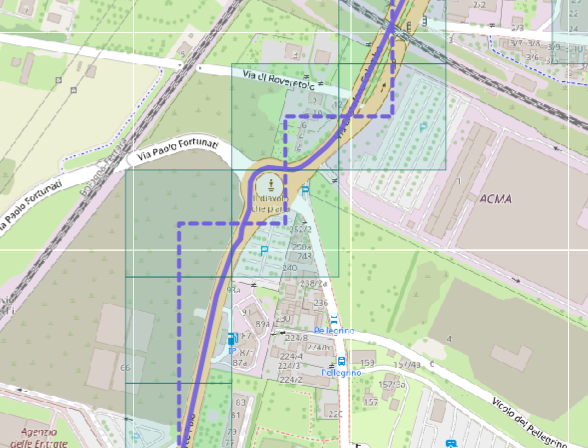
\includegraphics[width=\columnwidth]{privacy_grid_example.png}
\caption{Esempio su dati reali di un viaggio in auto: la linea
continua è il percorso realmente registrato; la linea tratteggiata è
la vista \emph{approximate} (griglia da 150\,m) dello stesso percorso.}
\label{fig:privacy-grid-example}
\end{figure}

Per valutare quantitativamente l'effetto di questa trasformazione,
vengono calcolate due metriche per ciascuna traccia. La
\emph{Privacy Perturbation} è la distanza media e massima, calcolata
con la formula di haversine, tra ciascun punto originale e il
corrispondente punto pubblicato dopo l'approssimazione a griglia. La
\emph{Quality of Service} è invece misurata come errore relativo tra
la lunghezza geodetica del percorso originale e quella del percorso
pubblicato,ed esprime quanto la generalizzazione spaziale distorce la
distanza realmente percorsa. Queste due metriche, calcolate per i tre
livelli di privacy, sono quelle riportate nella valutazione del
compromesso privacy/utilità in Sezione~\ref{sec:results}.

\subsubsection{Costruzione del diario in base al livello di privacy}

I tre livelli di privacy incidono sulla rappresentazione geografica e
sul dettaglio con cui vengono descritti i luoghi. Gli orari di inizio e
fine dei segmenti restano invece invariati in tutti i livelli. Nella
vista \emph{precise} nessun dato viene trasformato:
ogni segmento mostra l'orario esatto di inizio e fine, il percorso
GPS realmente registrato e, di conseguenza, la distanza realmente
percorsa; per una sosta, viene mostrato il nome vero del luogo
abituale a cui è stata associata, se esiste.

Nella vista \emph{approximate}, il percorso mostrato non è più quello
realmente registrato ma quello ottenuto dopo l'approssimazione
a griglia descritta sopra: la distanza del segmento viene quindi
ricalcolata su questo percorso approssimato, non su quello vero. Il
nome del luogo associato a una sosta, invece, resta visibile come
nella vista precisa: poiché la posizione è già protetta
dall'approssimazione a griglia delle coordinate, mostrare anche il
nome del luogo non aggiunge un rischio significativo ulteriore.

La vista \emph{aggregated} applica la stessa trasformazione del
percorso della vista approssimata, ma con una griglia più larga
(400\,m anziché 150\,m), e in più nasconde anche l'identità dei
luoghi: al posto del nome del luogo abituale mostra solo la sua
categoria generica o un'etichetta neutra se la sosta non è associata a
nessun luogo confermato.

\section{Risultati}
\label{sec:results}

\subsection{Valutazione del riconoscimento HAR}
\label{sec:har-results}

Le valutazioni usano il validation set ufficiale SHL~\cite{wang2018shl},
mai impiegato per aggiornare i pesi. La Tabella~\ref{tab:har-variants}
distingue la linea sperimentale dal modello realmente distribuito.

\begin{table}[htbp]
\caption{Confronto delle varianti CNN+GRU sul validation set ufficiale}
\centering
\scriptsize
\begin{tabular}{|l|c|c|r|}
\hline
\textbf{Variante} & \textbf{Canali} & \textbf{Sequenza} & \textbf{Accuracy} \\
\hline
Produzione originale & 6 & 32 & 79,47\% \\
\hline
Produzione distribuita & 6 & 128 & 84,88\% \\
\hline
\end{tabular}
\label{tab:har-variants}
\end{table}

Le due varianti condividono lo stesso checkpoint CNN+GRU: cambia solo
la lunghezza di sequenza usata in valutazione, non i pesi.

Poiché i pesi della GRU non dipendono dalla lunghezza della sequenza con
cui viene interrogata -- il layer applica la stessa trasformazione a
ogni passo, indipendentemente da quanti passi compongono la sequenza --
lo stesso checkpoint è stato valutato a più lunghezze di sequenza, per
osservare l'andamento dell'accuratezza e verificare se il guadagno
osservato passando da 32 a 128 continui, si stabilizzi o si inverta
per lunghezze ancora maggiori. La Tabella~\ref{tab:har-seqlen-sweep} e
la Figura~\ref{fig:har-seqlen-sweep} riportano l'andamento misurato
sul validation set ufficiale (115.156 finestre).

\begin{table}[htbp]
\caption{Accuratezza del modello distribuito al variare della lunghezza di sequenza}
\centering
\scriptsize
\begin{tabular}{|c|r|}
\hline
\textbf{Lunghezza sequenza} & \textbf{Accuracy} \\
\hline
32  & 79,46\% \\
\hline
64  & 82,50\% \\
\hline
128 & 84,88\% \\
\hline
256 & 86,08\% \\
\hline
512 & 86,38\% \\
\hline
\end{tabular}
\label{tab:har-seqlen-sweep}
\end{table}

\begin{figure}[htbp]
\centering
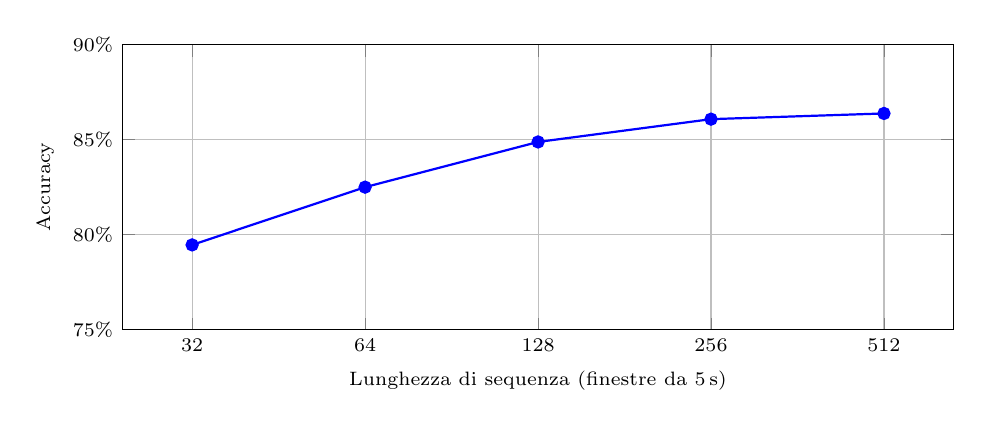
\begin{tikzpicture}
\begin{semilogxaxis}[
  width=\columnwidth,
  height=5.2cm,
  xlabel={Lunghezza di sequenza (finestre da 5\,s)},
  ylabel={Accuracy},
  log basis x={2},
  xtick={32,64,128,256,512},
  xticklabels={32,64,128,256,512},
  ymin=75, ymax=90,
  ytick distance=5,
  yticklabel={\pgfmathprintnumber{\tick}\%},
  tick label style={font=\scriptsize},
  label style={font=\scriptsize},
  grid=major,
]
\addplot[mark=*, blue, thick] coordinates {
  (32,79.46)
  (64,82.50)
  (128,84.88)
  (256,86.08)
  (512,86.38)
};
\end{semilogxaxis}
\end{tikzpicture}
\caption{Accuratezza sul validation set ufficiale al variare della
lunghezza di sequenza data in ingresso alla GRU, a parità di pesi
(nessun riaddestramento).}
\label{fig:har-seqlen-sweep}
\end{figure}

Il guadagno è marcato passando da 32 a 128 finestre (+5,4 punti), poi
si riduce progressivamente (128$\to$256: +1,2 punti; 256$\to$512: +0,3
punti) senza però invertirsi: fino a 512 finestre (~43 minuti di
contesto) l'accuratezza continua a salire, sia pure con rendimenti
marginali decrescenti. Non si osserva quindi, in questo intervallo, il
plateau o il lieve calo ipotizzato oltre i 256; la scelta di 128 per la
produzione resta un compromesso guidato dal costo di latenza (la GRU
bidirezionale non scala linearmente su CPU), non dal raggiungimento di
un punto di saturazione dell'accuratezza.

Questo guadagno di accuratezza da solo non giustifica però un
aumento di $L$ in produzione: la latenza è stata misurata direttamente
sul codice e sul modello reali (\texttt{HARClassifier}, stesso metodo
della Tabella~\ref{tab:har-latency} -- stesso processo, a caldo, stessi
input), per ciascuna lunghezza di sequenza e per dimensioni di
richiesta realistiche.

\begin{table}[htbp]
\caption{Latenza di HARClassifier al variare della lunghezza di sequenza (ms)}
\centering
\scriptsize
\begin{tabular}{|c|r|r|r|r|r|}
\hline
\textbf{L} & \textbf{100} & \textbf{500} & \textbf{1000} & \textbf{2000} & \textbf{Warmup} \\
\hline
32  & 81,7  & 131,0 & 567,0 & 921,7  & 7,2\,s \\
\hline
64  & 87,4  & 211,3 & 659,4 & 1186,0 & 15,0\,s \\
\hline
128 & 130,9 & 265,9 & 507,0 & 1212,7 & 30,4\,s \\
\hline
256 & 345,2 & 404,1 & 947,0 & 1479,1 & 73,2\,s \\
\hline
512 & 605,1 & 518,3 & 982,5 & 1299,5 & 166,2\,s \\
\hline
\end{tabular}
\label{tab:har-seqlen-latency}
\end{table}

Il costo di avvio (\emph{warmup}, la compilazione del grafo effettuata
una volta per processo worker) cresce da 30,4\,s a 128 finestre a
166,2\,s a 512, un fattore 5,5$\times$. Sulla dimensione di richiesta
più piccola (100 finestre), la latenza a caldo passa da 130,9\,ms a
605,1\,ms, un fattore 4,6$\times$. A fronte di questi costi, il
guadagno di 1,5 punti di accuratezza rispetto a 128 non è sufficiente
a giustificare il passaggio a $L=512$ in produzione: la scelta di
$L=128$ resta motivata dal costo di latenza, ora misurato direttamente
e non solo ipotizzato, e non da un plateau di accuratezza già
raggiunto.

Per valutare il modello distribuito sono state usate 115.156 finestre.
I valori grezzi dei primi sei canali sono stati ripristinati dal
tensore normalizzato prima dell'inferenza.

Le sequenze sono state costruite separatamente per ciascuna delle
quattro posizioni corporee. In questo modo il contesto della GRU non
attraversa registrazioni indipendenti.

L'accuracy è 84,88\%. Precision, recall e F1 macro sono 87,67\%,
77,12\% e 80,08\%; le corrispondenti medie pesate sono 85,60\%,
84,88\% e 84,30\%.

\begin{table*}[htbp]
\caption{Metriche per classe del modello CNN+GRU a sei canali distribuito in produzione}
\centering
\scriptsize
\begin{tabular}{|l|r|r|r|r|}
\hline
\textbf{Classe} & \textbf{Supporto} & \textbf{Precision} & \textbf{Recall} & \textbf{F1} \\
\hline
IDLE & 23.856 & 0,737 & 0,855 & 0,792 \\
WALKING & 20.920 & 0,848 & 0,946 & 0,894 \\
RUNNING & 2.220 & 0,998 & 0,754 & 0,859 \\
BIKING & 9.624 & 0,906 & 0,414 & 0,569 \\
MOVING\_VEHICLE & 58.536 & 0,894 & 0,887 & 0,890 \\
\hline
\end{tabular}
\label{tab:har-metrics}
\end{table*}

\begin{table*}[htbp]
\caption{Confusion matrix del modello CNN+GRU a sei canali distribuito; righe reali e colonne predette}
\centering
\scriptsize
\begin{tabular}{|l|r|r|r|r|r|}
\hline
\textbf{Reale $\backslash$ predetta} & \textbf{IDLE} & \textbf{WALK} & \textbf{RUN} & \textbf{BIKE} & \textbf{VEHICLE} \\
\hline
IDLE & 20.395 & 346 & 0 & 106 & 3.009 \\
WALKING & 626 & 19.786 & 3 & 92 & 413 \\
RUNNING & 0 & 332 & 1.674 & 213 & 1 \\
BIKING & 301 & 2.581 & 0 & 3.989 & 2.753 \\
MOVING\_VEHICLE & 6.346 & 285 & 0 & 2 & 51.903 \\
\hline
\end{tabular}
\label{tab:har-confusion}
\end{table*}

L'errore dominante è la confusione tra \texttt{IDLE} e
\texttt{MOVING\_VEHICLE}. Un veicolo fermo a un semaforo o nel traffico
può produrre un segnale simile a quello di una persona ferma.

La classe \texttt{BIKING} ha recall 0,414: viene confusa soprattutto
con \texttt{WALKING} e \texttt{MOVING\_VEHICLE}. \texttt{RUNNING} ha
precision 0,998 ma recall 0,754, anche per il supporto ridotto.

\subsection{Discussione dei casi ambigui}
\label{sec:har-ambiguous}

La confusion matrix (Tabella~\ref{tab:har-confusion}) permette di
analizzare quantitativamente alcuni casi che la sola accuracy
nasconderebbe.

\subsubsection{Veicolo fermo nel traffico o a un semaforo}

È il caso ambiguo
più frequente: 3.009 finestre reali \texttt{IDLE} vengono classificate
come \texttt{MOVING\_VEHICLE} e, simmetricamente, 6.346 finestre reali
\texttt{MOVING\_VEHICLE} vengono classificate come \texttt{IDLE}. Il
segnale accelerometrico e giroscopico di un veicolo fermo è infatti
indistinguibile, su una singola finestra di 5\,s, da quello di una
persona ferma: l'informazione che li distingue -- una velocità media
diversa da zero nei minuti circostanti -- esiste solo a livello di
sequenza, non di singola finestra isolata.

\subsubsection{Cammino veloce confuso con la bicicletta}

\texttt{BIKING} ha
il recall più basso del modello (0,414): 2.581 finestre reali di
bicicletta vengono classificate come \texttt{WALKING} e 2.753 come
\texttt{MOVING\_VEHICLE}. Un cammino sostenuto o una discesa in
bicicletta a bassa velocità producono profili di accelerazione
sovrapposti, e \texttt{BIKING} ha inoltre il supporto più basso tra le
classi frequenti (9.624 finestre), rendendo il confine di decisione
meno stabile.

\subsubsection{Fermate temporanee durante uno spostamento}

Una sosta breve
(es. attesa a un incrocio durante una camminata) può generare qualche
finestra isolata classificata \texttt{IDLE} in mezzo a una sequenza
altrimenti \texttt{WALKING}. A livello di singola finestra questo è un
errore locale coerente con l'analisi precedente; la segmentazione del
diario (Sezione~\ref{sec:implementation}) non lo propaga come sosta a
sé stante, perché riassegna all'etichetta circostante ogni gruppo di
finestre con etichetta diversa che duri meno di 60\,s
(Figura~\ref{fig:isolated-label}) -- una finestra isolata non genera
quindi una sosta spuria nel diario finale.

\subsubsection{Cambio di mezzo di trasporto}

Un cambio reale di modalità
(es. da \texttt{WALKING} a \texttt{MOVING\_VEHICLE} salendo su un
autobus) produce necessariamente alcune finestre di transizione
ambigue nell'intorno del cambio, mentre il segnale sensoriale converge
verso il nuovo pattern di moto. Questo caso va distinto dal
precedente: non viene rimosso dallo smoothing (è un cambio reale, non
rumore da correggere), ma diventa il confine tra due segmenti del
diario non appena la sequenza di etichette si stabilizza nella nuova
modalità.

La Tabella~\ref{tab:har-latency} confronta le pipeline nello stesso
processo, a caldo e sugli stessi input. La fusione del modello e la
chiamata in batch riducono il costo senza cambiare i pesi.

\begin{table}[htbp]
\caption{Latenza dell'inferenza, pipeline originale e ottimizzata}
\centering
\scriptsize
\begin{tabular}{|r|r|r|r|}
\hline
\textbf{Finestre} & \textbf{Originale} & \textbf{Ottimizzata} & \textbf{Speedup} \\
\hline
141 & 110,9\,ms & 42,1\,ms & 2,6$\times$ \\
579 & 410,6\,ms & 93,6\,ms & 4,4$\times$ \\
1060 & 728,2\,ms & 145,8\,ms & 5,0$\times$ \\
\hline
\end{tabular}
\label{tab:har-latency}
\end{table}

Sull'intero validation set la pipeline passa da 68,4\,s a 25,7\,s,
uno speedup di 2,7$\times$. L'accuracy passa dal 79,47\% della
configurazione originale al valore distribuito di 84,88\%.

Il guadagno di velocità deriva dal pattern di chiamata; quello di
accuratezza dal contesto più lungo. Sono quindi due effetti distinti.

\subsection{Compromesso privacy/utilità}

Le metriche di Privacy Perturbation e Quality of Service definite in
Sezione~\ref{sec:implementation} sono state calcolate sull'insieme dei
viaggi realmente registrati nel database, segmento per segmento:
separatamente per i segmenti di movimento, raggruppati per modalità
di attività riconosciuta, e per i segmenti di sosta, per cui la
perturbazione è calcolata sul centroide GPS della sosta anziché sulla
lunghezza di un percorso. La Tabella~\ref{tab:privacy-results}
riporta i risultati.

\begin{table}[htbp]
\caption{Privacy Perturbation media e Quality of Service (errore
relativo di distanza) per modalità, sui due livelli protetti}
\centering
\scriptsize
\begin{tabular}{|l|r|c|c|c|c|}
\hline
\multirow{2}{*}{\textbf{Modalità}} & \multirow{2}{*}{\textbf{n}} &
\multicolumn{2}{c|}{\textbf{Perturbation (m)}} &
\multicolumn{2}{c|}{\textbf{QoS (err. rel.)}} \\
\cline{3-6}
 & & \textbf{approx.} & \textbf{aggr.} & \textbf{approx.} & \textbf{aggr.} \\
\hline
Veicolo & 38 & 37,3 & 100,3 & 0,64 & 0,61 \\
\hline
A piedi & 56 & 41,9 & 93,0 & 0,93 & 1,06 \\
\hline
Bicicletta & 3 & 44,8 & 82,3 & 0,50 & 1,28 \\
\hline
Sosta & 51 & 35,7 & 97,5 & -- & -- \\
\hline
\end{tabular}
\label{tab:privacy-results}
\end{table}

\begin{figure*}[htbp]
\centering
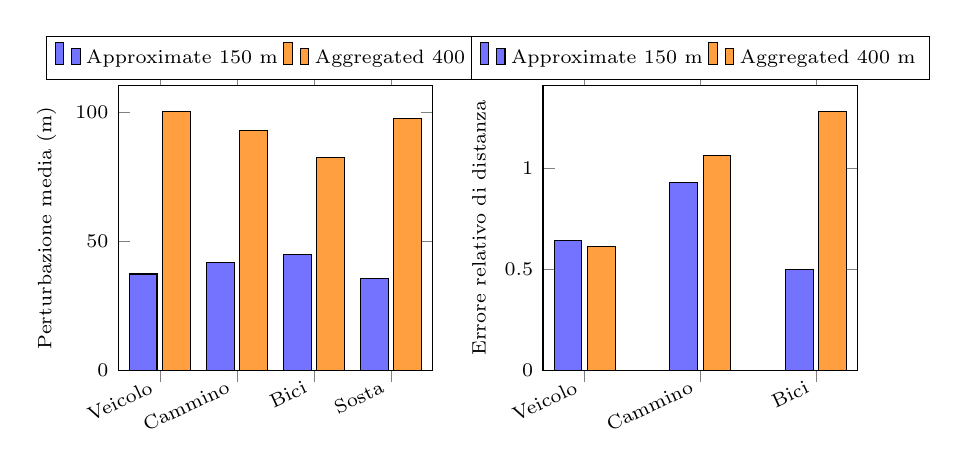
\begin{tikzpicture}
\begin{groupplot}[
  group style={group size=2 by 1, horizontal sep=1.4cm},
  width=0.46\textwidth,
  height=5.2cm,
  ybar,
  ymin=0,
  enlarge x limits=0.18,
  symbolic x coords={Veicolo,Cammino,Bici,Sosta},
  xtick=data,
  x tick label style={rotate=25,anchor=east,font=\scriptsize},
  tick label style={font=\scriptsize},
  label style={font=\scriptsize},
  legend style={font=\scriptsize,at={(0.5,1.02)},anchor=south,legend columns=2},
]
\nextgroupplot[
  ylabel={Perturbazione media (m)},
  title={Privacy Perturbation},
  title style={font=\small},
]
\addplot[fill=blue!55] coordinates {
  (Veicolo,37.3) (Cammino,41.9) (Bici,44.8) (Sosta,35.7)
};
\addplot[fill=orange!75] coordinates {
  (Veicolo,100.3) (Cammino,93.0) (Bici,82.3) (Sosta,97.5)
};
\legend{Approximate 150 m,Aggregated 400 m}

\nextgroupplot[
  ylabel={Errore relativo di distanza},
  title={Quality of Service},
  title style={font=\small},
  symbolic x coords={Veicolo,Cammino,Bici},
]
\addplot[fill=blue!55] coordinates {
  (Veicolo,0.64) (Cammino,0.93) (Bici,0.50)
};
\addplot[fill=orange!75] coordinates {
  (Veicolo,0.61) (Cammino,1.06) (Bici,1.28)
};
\legend{Approximate 150 m,Aggregated 400 m}
\end{groupplot}
\end{tikzpicture}
\caption{Trade-off misurato tra protezione della posizione e utilità.
La griglia più ampia aumenta sempre la perturbazione, mentre la
distorsione della distanza dipende dalla geometria e dalla lunghezza
tipica dei segmenti di ciascuna modalità.}
\label{fig:privacy-qos-tradeoff}
\end{figure*}

La Privacy Perturbation cresce con la dimensione della cella, come
atteso: passando da \emph{approximate} (150\,m) ad \emph{aggregated}
(400\,m) la distanza media tra punto reale e punto pubblicato più che
raddoppia in tutte le modalità, comprese le soste. La Quality of
Service, invece, non peggiora sempre in modo monotono con
l'aggregazione: per i segmenti in auto l'errore relativo di distanza è
leggermente più basso con celle più grandi (0,61 contro 0,64) che con
celle più piccole.
Il campione di segmenti in bicicletta è troppo piccolo (\emph{n}=3) per trarne conclusioni robuste, ed è
riportato solo per completezza.

\subsection{Latenza della pipeline di ingestione}

Per misurare il tempo impiegato dalle diverse fasi della pipeline di
caricamento ed elaborazione di un viaggio è stato eseguito un test di
carico con un client sintetico che riproduce il comportamento
dell'applicazione mobile reale (Sezione~\ref{sec:implementation}).
Sono stati simulati 25 utenti che caricano contemporaneamente viaggi
di circa un'ora: poiché un utente non può avere più di un viaggio in
corso alla volta (Sezione~\ref{sec:implementation}), ciascuno ha
caricato i propri viaggi in sequenza, uno alla volta, per un totale
di 10 viaggi a testa (250 viaggi complessivi). La fase di upload raw è
stata cronometrata lato client; le altre quattro fasi, lato backend.
Il test è stato eseguito su un
ambiente locale equivalente a quello di produzione (stessi container
Docker), non sull'hardware di produzione stesso: i valori assoluti
vanno quindi letti come indicativi, mentre le proporzioni relative
tra le fasi restano informative.

\begin{table}[htbp]
\caption{Latenza media delle fasi della pipeline di ingestione (250 viaggi, 25 utenti concorrenti)}
\centering
\scriptsize
\begin{tabular}{|l|r|r|r|r|}
\hline
\textbf{Fase} & \textbf{Media} & \textbf{Dev.std} & \textbf{Min} & \textbf{Max} \\
\hline
Core (GPS+transizioni) & 2,02\,s & 2,61\,s & 0,25\,s & 15,83\,s \\
\hline
Upload raw (client) & 3,04\,s & 2,56\,s & 0,43\,s & 28,59\,s \\
\hline
HAR + diario & 4,62\,s & 1,50\,s & 1,99\,s & 11,06\,s \\
\hline
Batch insert raw & 29,68\,s & 8,235\,s & 20,39\,s & 53,97\,s \\
\hline
Data mining luoghi & 0,97\,s & 0,64\,s & 0,27\,s & 2,74\,s \\
\hline
\end{tabular}
\label{tab:pipeline-latency}
\end{table}

La fase nettamente più onerosa è l'inserimento in batch dei dati
sensoriali grezzi (media 29,68\,s, fino a quasi 1 minuto nel caso
peggiore), dovuto al volume di righe scritte in
\texttt{RawSensorReading} -- una per ogni campione, quindi fino a
360.000 righe per un singolo viaggio di un'ora (720 finestre da 500
campioni). L'inserimento usa già \texttt{bulk\_create} a gruppi di
5000 righe (72 batch per un viaggio di un'ora), quindi il costo non
è dovuto a query singole per riga, ma al volume assoluto di dati
scritti a questa granularità, aggravato dalla contesa sul database
sotto 25 utenti concorrenti. 
Va però notato che il batch insert dei dati grezzi non è una fase
percepita dall'utente: il diario del viaggio è già disponibile non
appena termina la fase HAR, mentre la persistenza dei dati grezzi
prosegue in background. La latenza effettivamente percepita
dall'utente -- core, upload raw e HAR/diario -- resta quindi
complessivamente bassa, dell'ordine di pochi secondi.

Per correttezza va infine segnalato che la velocità della fase HAR
è in parte dovuta al fatto che il modello viene caricato in memoria
una sola volta all'avvio di ciascun processo worker Celery
(\texttt{warm\_har\_model\_on\_worker\_start}, agganciato al segnale
\texttt{worker\_process\_init}), anziché ad ogni singola richiesta di
inferenza. Questo rende l'inferenza rapida a runtime, ma ha come
contropartita un utilizzo di RAM elevato per ciascun worker, dato il
peso del modello tenuto costantemente in memoria.

Questo suggerisce due direzioni per un'eventuale scalatura del
sistema oltre il semplice aumento del numero di worker. La prima
riguarda proprio il modello HAR: passare da una copia caricata in
RAM per ciascun worker a un'unica istanza condivisa, interrogata dai
worker come servizio separato, ridurrebbe l'occupazione di memoria
aggregata a scapito di una latenza leggermente più alta sulla
singola richiesta di inferenza -- un compromesso favorevole quando
l'obiettivo è aumentare il numero di worker eseguibili in parallelo
sulla stessa macchina. La seconda riguarda il database: durante il
test di carico è stato il componente più sollecitato in assoluto (più
dei worker Celery stessi), per cui scalare orizzontalmente il sistema
richiederebbe anche di replicare il database e introdurre una logica
di sincronizzazione tra le repliche, oltre alla sola duplicazione dei
worker applicativi.

\subsection*{Dichiarazione sull'utilizzo di strumenti di Intelligenza Artificiale}

Nello sviluppo di questo progetto è stato utilizzato Claude (Anthropic),
tramite l'interfaccia Claude Code, in due ambiti distinti.

\subsubsection{Confronto e ricerca}

Lo strumento è stato usato come
supporto alla ricerca e al confronto di idee e scelte progettuali,
in particolare per
raccogliere e confrontare più fonti/approcci con relativi
pro e contro, in tempi più rapidi rispetto a una ricerca manuale
condotta fonte per fonte.

\subsubsection{Scrittura di codice}

Lo strumento è stato usato per:
\begin{itemize}
  \item supportare lo sviluppo dell'interfaccia grafica finale
  dell'applicazione mobile e della dashboard web;
  \item refactoring e pulizia del codice esistente, in particolare lato
  frontend/mobile, per farlo aderire il più possibile
  all'architettura scelta per il progetto;
  \item scrivere piccole porzioni di codice per gestire casi limite
  lato backend;
  \item scrittura dei DTO (Data Transfer Object) lato frontend, usati
  per mappare le risposte JSON delle API REST del backend nei modelli
  dati dell'applicazione mobile e della dashboard web.
\end{itemize}



La progettazione dell'architettura, la raccolta e l'elaborazione dei
dati, l'implementazione delle pipeline di training e valutazione del
modello HAR, e tutte le decisioni progettuali del sistema sono opera
dello studente, che dichiara di comprendere integralmente il codice e
i contenuti presentati in questa relazione.

\section*{Conclusione}

In questo lavoro ho presentato Mobility Diary, un sistema
context-aware per la costruzione di un diario personale di mobilità,
composto da un'applicazione mobile, un back-end che ne gestisce
l'elaborazione asincrona e una dashboard amministrativa. Il sistema
integra una macchina a stati finiti per il rilevamento del movimento,
un modulo di riconoscimento dell'attività umana basato su CNN1D e
GRU, e meccanismi di generalizzazione spaziale per proteggere la
posizione dell'utente su tre livelli di privacy.

Il modulo HAR raggiunge un'accuratezza dell'84,88\% sul validation set
ufficiale dopo l'ottimizzazione per l'inferenza in produzione. Sul
fronte privacy, l'analisi condotta sui viaggi realmente registrati
mostra che la Privacy Perturbation cresce in modo prevedibile con la
dimensione della cella di generalizzazione, mentre l'effetto
sull'utilità del dato varia a seconda della modalità di movimento: per
gli spostamenti in auto, tipicamente lunghi e rettilinei, la Quality
of Service resta pressoché stabile anche con la griglia più larga,
mentre per la camminata, fatta di percorsi più brevi, l'aggregazione
comporta una perdita di utilità più marcata.

Sul fronte delle prestazioni, il test di carico sulla pipeline di
ingestione mostra che la latenza effettivamente percepita
dall'utente -- upload dei dati e classificazione HAR, dopo la quale
il diario è già consultabile -- resta dell'ordine di pochi secondi,
mentre la persistenza dei dati sensoriali grezzi, molto più lenta,
avviene in background senza impatto percepito. Sotto carico
concorrente il database si conferma il componente più sollecitato,
indicando che una futura scalata del sistema richiederebbe la sua
replica, oltre a un modello HAR condiviso tra i worker invece che
duplicato in RAM su ciascuno.

Il sistema presenta comunque dei limiti. La macchina a stati finiti
che rileva il movimento è un'euristica costruita ad hoc su
accelerometro e GPS, ed è verosimilmente meno precisa delle API di
riconoscimento dell'attività fornite nativamente dal sistema
operativo del telefono, che non sono state utilizzate. Il modulo HAR,
inoltre, non distingue tra le diverse modalità di trasporto
motorizzato -- auto, autobus, treno -- che vengono tutte classificate
in un'unica etichetta \texttt{MOVING\_VEHICLE}.

Due direzioni di sviluppo futuro appaiono particolarmente rilevanti.
La prima è l'introduzione di un processo periodico che elimini dallo
storage a oggetti i dati sensoriali grezzi di un viaggio una volta che
la sua elaborazione è completata: attualmente questi dati non vengono
mai rimossi automaticamente, e restano nello storage indefinitamente
a meno che l'utente non cancelli esplicitamente il viaggio. La
seconda è un meccanismo con cui l'utente possa correggere le
etichette di attività assegnate dal modulo HAR quando errate (ad
esempio segnalando che un tratto indicato come cammino era in realtà
percorso in auto), e una pipeline che raccolga queste correzioni per
aggiornare periodicamente i pesi del modello.

\balance
\begin{thebibliography}{00}

\bibitem{wang2018shl}
``Sussex-Huawei Locomotion \& Transportation Dataset.'' [Online].
Available: \url{http://www.shl-dataset.org/}. Accessed: Sep. 14, 2026.

\bibitem{postgis-manual}
PostGIS Project, ``PostGIS Manual: Geography Data Type and
ST\_Length.'' [Online]. Available:
\url{https://postgis.net/docs/using_postgis_dbmanagement.html} and
\url{https://postgis.net/docs/ST_Length.html}. Accessed: Sep. 13, 2026.

\bibitem{timescale-hypertables}
Timescale, ``Hypertables,'' \emph{Timescale Documentation}. [Online].
Available: \url{https://docs.timescale.com/use-timescale/latest/hypertables/}.
Accessed: Sep. 13, 2026.

\bibitem{mapbox-directions}
Mapbox, ``Geocoding API and Directions API,'' \emph{Mapbox API
Documentation}. [Online]. Available:
\url{https://docs.mapbox.com/api/search/geocoding/} and
\url{https://docs.mapbox.com/api/navigation/directions/}.
Accessed: Sep. 13, 2026.

\bibitem{yang2015cnn}
J. Brownlee, ``1D Convolutional Neural Network Models for Human
Activity Recognition,'' \emph{Machine Learning Mastery}. [Online].
Available:
\url{https://machinelearningmastery.com/cnn-models-for-human-activity-recognition-time-series-classification/}.
Accessed: Sep. 14, 2026.

\bibitem{cho2014gru}
``Gated Recurrent Unit Networks,'' \emph{GeeksforGeeks}. [Online].
Available:
\url{https://www.geeksforgeeks.org/machine-learning/gated-recurrent-unit-networks/}.
Accessed: Sep. 14, 2026.

\bibitem{ester1996dbscan}
S. Yıldırım, ``DBSCAN Clustering -- Explained,'' \emph{Towards Data
Science}. [Online]. Available:
\url{https://towardsdatascience.com/dbscan-clustering-explained-97556a2ad556/}.
Accessed: Sep. 14, 2026.

\bibitem{gruteser2003cloaking}
``Spatial Cloaking,'' \emph{Wikipedia}. [Online]. Available:
\url{https://en.wikipedia.org/wiki/Spatial_cloaking}. Accessed:
Sep. 14, 2026.

\bibitem{pine-architecture}
A. Avvenuti, ``Pine: A Lightweight Architecture Helper for your
Flutter Projects,'' \emph{Medium}. [Online]. Available:
\url{https://angeloavv.medium.com/pine-a-lightweight-architecture-helper-for-your-flutter-projects-1ce69ac63f74}.
Accessed: Sep. 14, 2026.

\end{thebibliography}

\end{document}
